\documentclass[10.5pt,a4paper,openany]{book}
\usepackage[a4paper,margin=20mm,headheight=15pt]{geometry}
\usepackage{fontspec}
\setmainfont{DejaVu Serif}
\setsansfont{DejaVu Sans}
\setmonofont{DejaVu Sans Mono}[Scale=0.84]
\usepackage{microtype}
\usepackage{xcolor}
\definecolor{UGTSNavy}{HTML}{0B2638}
\definecolor{UGTSTeal}{HTML}{168F9C}
\definecolor{UGTSGold}{HTML}{D8A124}
\definecolor{UGTSCoral}{HTML}{D76959}
\definecolor{UGTSPurple}{HTML}{786AA3}
\definecolor{UGTSGreen}{HTML}{2A8C6D}
\definecolor{UGTSLight}{HTML}{EDF4F5}
\definecolor{UGTSGray}{HTML}{60747C}
\definecolor{UGTSDark}{HTML}{1A2E38}
\usepackage{graphicx}
\graphicspath{{../diagrams/}}
\usepackage{booktabs,longtable,tabularx,array}
\usepackage{ragged2e,pdflscape}
\newcolumntype{L}[1]{>{\RaggedRight\arraybackslash}p{#1}}
\setlength{\tabcolsep}{3pt}
\renewcommand{\arraystretch}{1.15}
\usepackage{amsmath,amssymb,mathtools}
\usepackage{enumitem}
\setlist{nosep,leftmargin=1.5em}
\usepackage[most]{tcolorbox}
\usepackage{listings}
\usepackage{caption}
\usepackage{float}
\usepackage{fancyhdr}
\usepackage{titlesec}
\usepackage{hyperref}
\usepackage{xurl}
\usepackage{lastpage}
\usepackage{needspace}
\hypersetup{colorlinks=true,linkcolor=UGTSTeal,urlcolor=UGTSPurple,citecolor=UGTSCoral,pdfauthor={OpenAI synthesis of user-supplied corpus},pdftitle={Unified Geometric-Topological Substrate}}
\pagestyle{fancy}
\fancyhf{}
\fancyhead[L]{\sffamily\small Unified Geometric-Topological Substrate}
\fancyhead[R]{\sffamily\small UGTS-0}
\fancyfoot[L]{\sffamily\scriptsize Source extraction + bounded engineering normalization}
\fancyfoot[R]{\sffamily\scriptsize \thepage\ / \pageref{LastPage}}
\renewcommand{\headrulewidth}{0.3pt}
\renewcommand{\footrulewidth}{0pt}
\titleformat{\chapter}[display]{\sffamily\bfseries\color{UGTSNavy}}{\fontsize{14}{16}\selectfont PART \thechapter}{5pt}{\fontsize{26}{30}\selectfont}
\titleformat{\section}{\sffamily\bfseries\Large\color{UGTSNavy}}{\thesection}{0.7em}{}
\titleformat{\subsection}{\sffamily\bfseries\large\color{UGTSTeal}}{\thesubsection}{0.7em}{}
\titleformat{\subsubsection}{\sffamily\bfseries\color{UGTSDark}}{\thesubsubsection}{0.7em}{}
\titlespacing*{\chapter}{0pt}{-15pt}{18pt}
\setcounter{tocdepth}{2}
\setcounter{secnumdepth}{3}

\newcommand{\statusretain}{\tcbox[on line,boxsep=1pt,left=3pt,right=3pt,top=1pt,bottom=1pt,arc=2pt,colback=UGTSTeal,colframe=UGTSTeal,coltext=white,fontupper=\sffamily\bfseries\scriptsize]{RETAIN}}
\newcommand{\statustranslate}{\tcbox[on line,boxsep=1pt,left=3pt,right=3pt,top=1pt,bottom=1pt,arc=2pt,colback=UGTSGold,colframe=UGTSGold,coltext=UGTSNavy,fontupper=\sffamily\bfseries\scriptsize]{TRANSLATE}}
\newcommand{\statusdemote}{\tcbox[on line,boxsep=1pt,left=3pt,right=3pt,top=1pt,bottom=1pt,arc=2pt,colback=UGTSPurple,colframe=UGTSPurple,coltext=white,fontupper=\sffamily\bfseries\scriptsize]{DEMOTE}}
\newcommand{\statuscorrect}{\tcbox[on line,boxsep=1pt,left=3pt,right=3pt,top=1pt,bottom=1pt,arc=2pt,colback=UGTSPurple,colframe=UGTSPurple,coltext=white,fontupper=\sffamily\bfseries\scriptsize]{CORRECT}}
\newcommand{\statusreject}{\tcbox[on line,boxsep=1pt,left=3pt,right=3pt,top=1pt,bottom=1pt,arc=2pt,colback=UGTSCoral,colframe=UGTSCoral,coltext=white,fontupper=\sffamily\bfseries\scriptsize]{REJECT}}
\newcommand{\src}[1]{\textcolor{UGTSPurple}{\sffamily\bfseries Source #1}}
\newcommand{\code}[1]{\texttt{#1}}
\newcommand{\term}[1]{\textbf{#1}}

\newtcolorbox{sourcebox}[1][]{enhanced,breakable,colback=UGTSLight,colframe=UGTSTeal,title={SOURCE-DERIVED},fonttitle=\sffamily\bfseries,#1}
\newtcolorbox{normalbox}[1][]{enhanced,breakable,colback=white,colframe=UGTSGold,title={ENGINEERING NORMALIZATION},fonttitle=\sffamily\bfseries,coltitle=UGTSNavy,#1}
\newtcolorbox{riskbox}[1][]{enhanced,breakable,colback=red!3,colframe=UGTSCoral,title={BOUNDARY / RISK},fonttitle=\sffamily\bfseries,#1}
\newtcolorbox{decisionbox}[1][]{enhanced,breakable,colback=UGTSNavy,colframe=UGTSNavy,coltext=white,title={DECISION},fonttitle=\sffamily\bfseries,coltitle=UGTSGold,#1}
\newtcolorbox{examplebox}[1][]{enhanced,breakable,colback=green!3,colframe=UGTSGreen,title={WORKED EXAMPLE},fonttitle=\sffamily\bfseries,#1}

\lstdefinestyle{ugts}{basicstyle=\ttfamily\small,breaklines=true,breakatwhitespace=false,columns=fullflexible,keepspaces=true,showstringspaces=false,frame=single,rulecolor=\color{UGTSGray},backgroundcolor=\color{UGTSLight},keywordstyle=\color{UGTSPurple}\bfseries,commentstyle=\color{UGTSGreen},stringstyle=\color{UGTSCoral},numbers=left,numberstyle=\tiny\color{UGTSGray},xleftmargin=1.5em,framexleftmargin=1.2em}
\lstset{style=ugts}

\begin{document}
\frontmatter
\begin{titlepage}
\pagecolor{UGTSNavy}
\color{white}
\vspace*{12mm}
{\sffamily\bfseries\fontsize{31}{35}\selectfont Unified Geometric-Topological Substrate\par}
\vspace{5mm}
{\sffamily\fontsize{17}{21}\selectfont A clean information architecture extracted from the supplied geometry, game-technology, graphics and topology corpus\par}
\vspace{13mm}
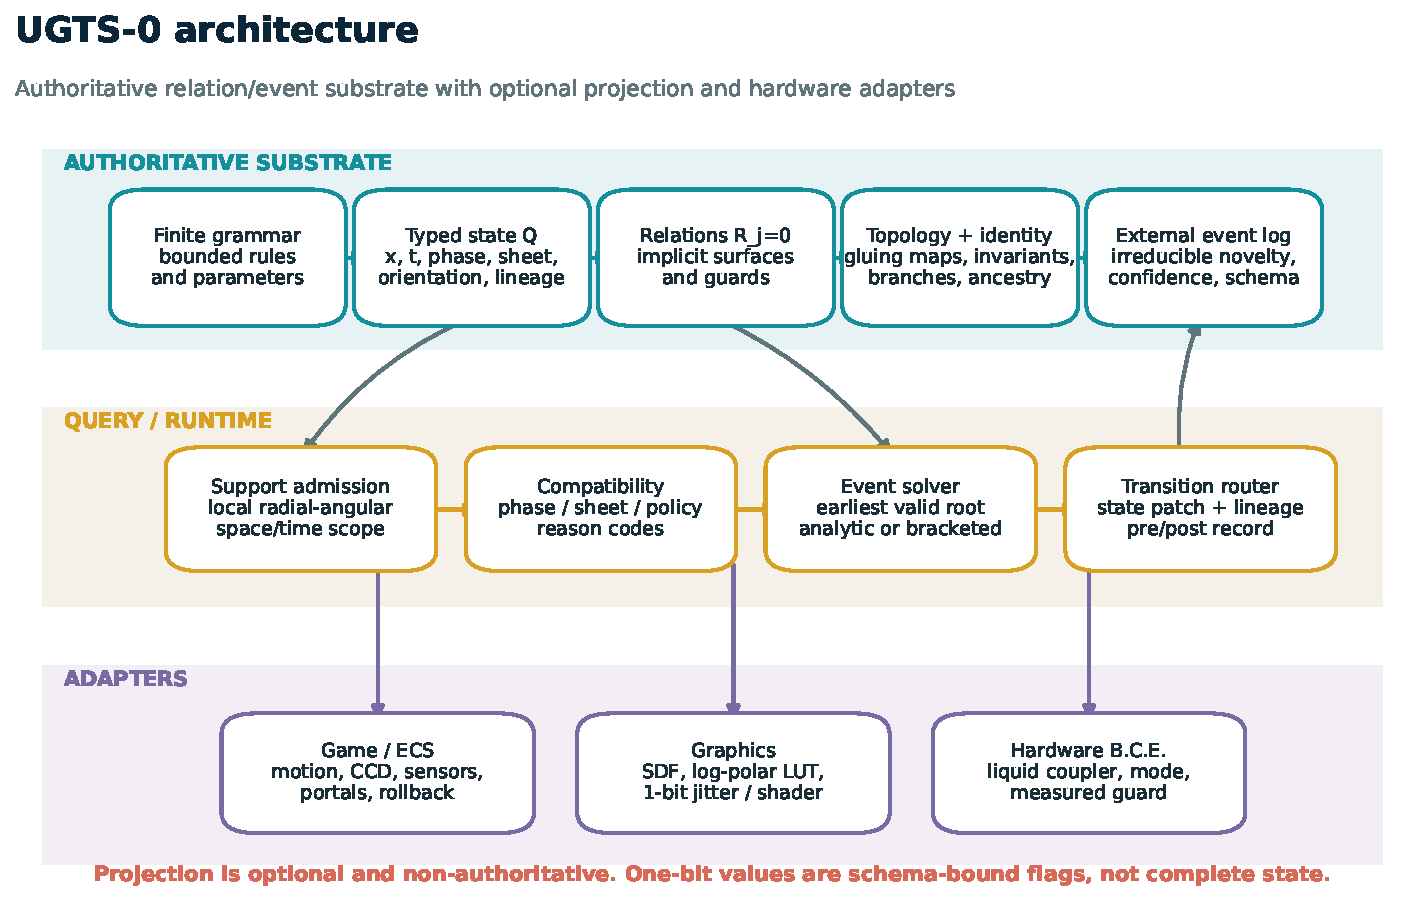
\includegraphics[width=\textwidth]{architecture_overview.pdf}
\vfill
\begin{tcolorbox}[colback=white!10!UGTSNavy,colframe=UGTSTeal,coltext=white,arc=3mm,boxrule=1pt]
\sffamily\large
\textbf{Deliverable:} technical synthesis, full concept inventory, claims ledger, formal specification, reference implementation, tests, examples, graphics shader, game-engine adapters and bounded optofluidic endpoint.
\end{tcolorbox}
\vspace{6mm}
{\sffamily\small Prepared from nine user-supplied PDFs. Personal identifiers were intentionally omitted from this synthesis.\par}
{\sffamily\small Version 1.0 - August 2026\par}
\end{titlepage}
\nopagecolor
\color{black}

\chapter*{Abstract}
\addcontentsline{toc}{chapter}{Abstract}
The supplied documents contain a recurring technical line beneath a large amount of metaphor and speculative extrapolation. The recoverable line is not a new rasterizer and not a claim that all reality is literally spherical. It is a \emph{query-first state-and-event substrate}: a finite grammar produces typed continuous state; local radial-angular supports select relevance; compatibility predicates decide whether co-located sectors may interact; relation surfaces define events; transitions update phase, sheet, orientation, branch and lineage; and an external event log records novelty that cannot be recomputed. Images, game-engine frames and optical devices are downstream adapters.

This report extracts 69 individual mechanisms, assigns each a disposition, and unifies the retained operators into \term{UGTS-0 / Equation World Zero}. The accompanying Python package implements typed state, linear/quadratic trajectories, implicit geometry, analytic and bracketed event solvers, radial-angular support, phase/sheet compatibility, Mobius and Klein quotient maps, four-chamber hourglass routing, log-polar bit lookup, finite grammars, optional 1-bit projection, and a measured Bounded Compatibility Event controller. Seventeen executable tests pass.

\begin{decisionbox}
The technically coherent core is: \textbf{finite grammar + typed state + local support + compatibility + event solving + transition + lineage + external log}. The strongest prototype is intentionally restricted. Universal O(1), zero-memory, zero-latency, physical Klein-bottle self-assembly, and one-bit-complete-state claims are rejected.
\end{decisionbox}

\tableofcontents
\listoffigures
\mainmatter

\chapter{Executive unification}
\section{The decisive shift}
\begin{sourcebox}
The mature synthesis in S6 says the archive should no longer be judged primarily as rasterization, raymarching, voxel storage or a frame-loop proposal. Cones, SDF-zero, one-bit, double vacuum and hourglass are recast as operators in a shared state space. Spherical structure is local support, shelling and radial reach, not a universal replacement for every world representation (S6, pp. 1--7).
\end{sourcebox}

\begin{normalbox}
UGTS-0 therefore treats the authoritative object as a relation/event world. A renderer may visualize the world, but the image is not the state. A game loop may schedule queries, but the loop is not the ontology. A one-bit field may route a transition, but it is not the amplitude, uncertainty, identity or geometry.
\end{normalbox}

The unified statement is:
\begin{quote}
A finite grammar generates a typed continuous state manifold. Local radial-angular supports define relevance and measurement. Events occur when a relation crosses an explicit transition surface while support and compatibility hold. Identity persists by lineage and invariants rather than by instantaneous coordinates. Projection into images, engine objects or photonic outputs is optional and non-authoritative.
\end{quote}

\begin{figure}[H]
\centering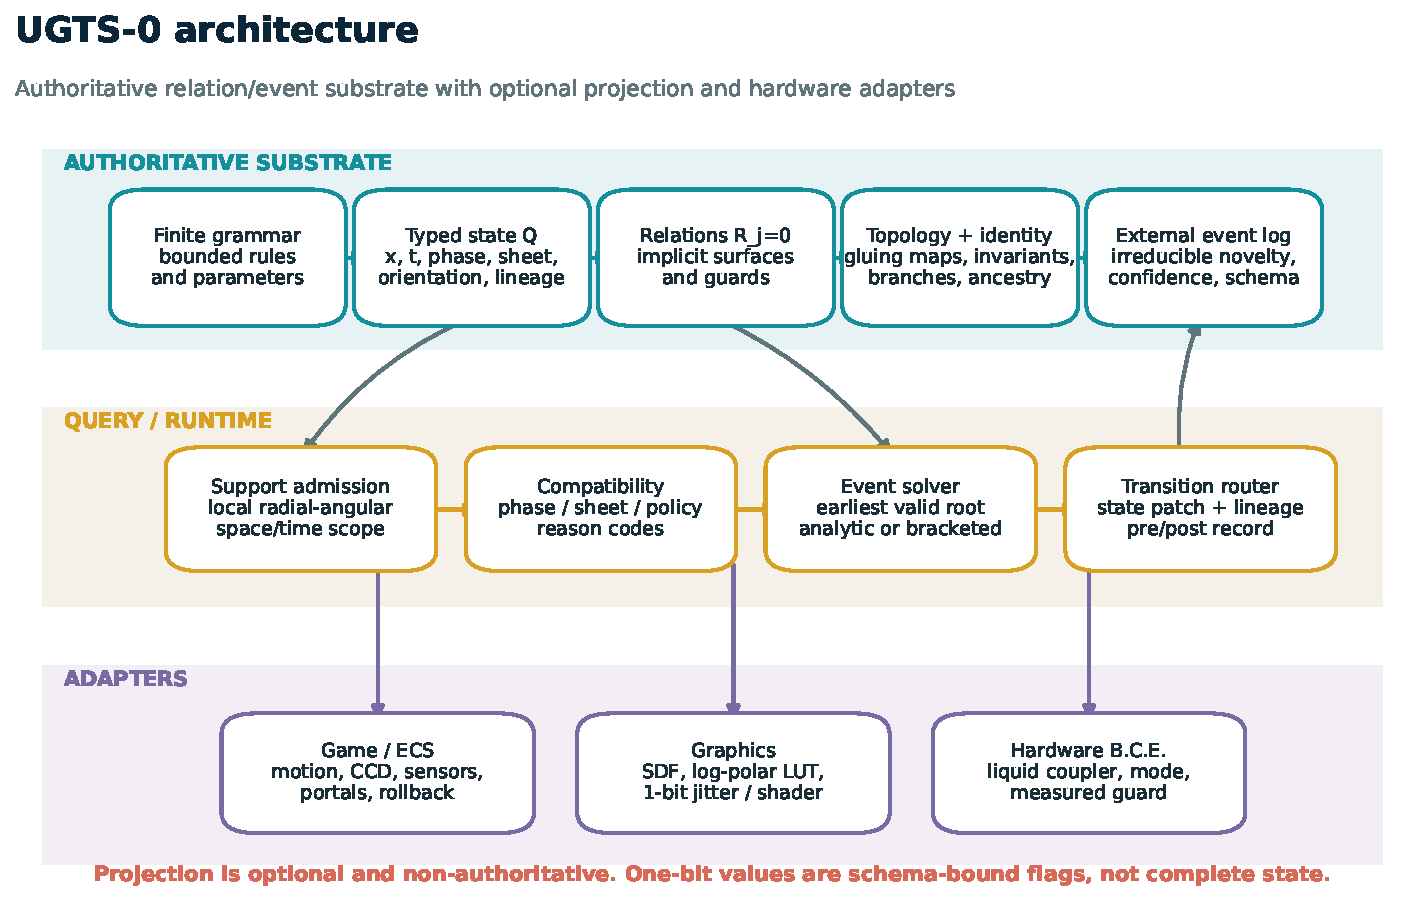
\includegraphics[width=\textwidth]{architecture_overview.pdf}
\caption{UGTS-0 separates authoritative substrate, query runtime and adapters.}
\end{figure}

\section{What ``works technically'' means here}
The package does not claim to solve every scene, PDE, physics problem or AI task. ``Works'' means the following bounded capabilities are executable and tested:
\begin{enumerate}
\item Evaluate closed-form entity state at an arbitrary continuous time.
\item Find the earliest valid crossing for supported surface/trajectory families.
\item Filter candidates by local radial-angular support and typed compatibility.
\item Apply explicit state patches while preserving pre-state, post-state and lineage.
\item Represent co-location without coupling by phase/sheet/orientation mismatch.
\item Apply Mobius, Klein, portal and hourglass maps as explicit software gluing/routing.
\item Use log-polar coordinates and a compact one-bit LUT as an optional local address mask.
\item Project implicit fields through an ordinary graphics adapter and posterize to one bit.
\item Run a measured B.C.E. threshold/compatibility controller with a narrow parity bit.
\end{enumerate}

\section{Retention rule}
\begin{figure}[H]
\centering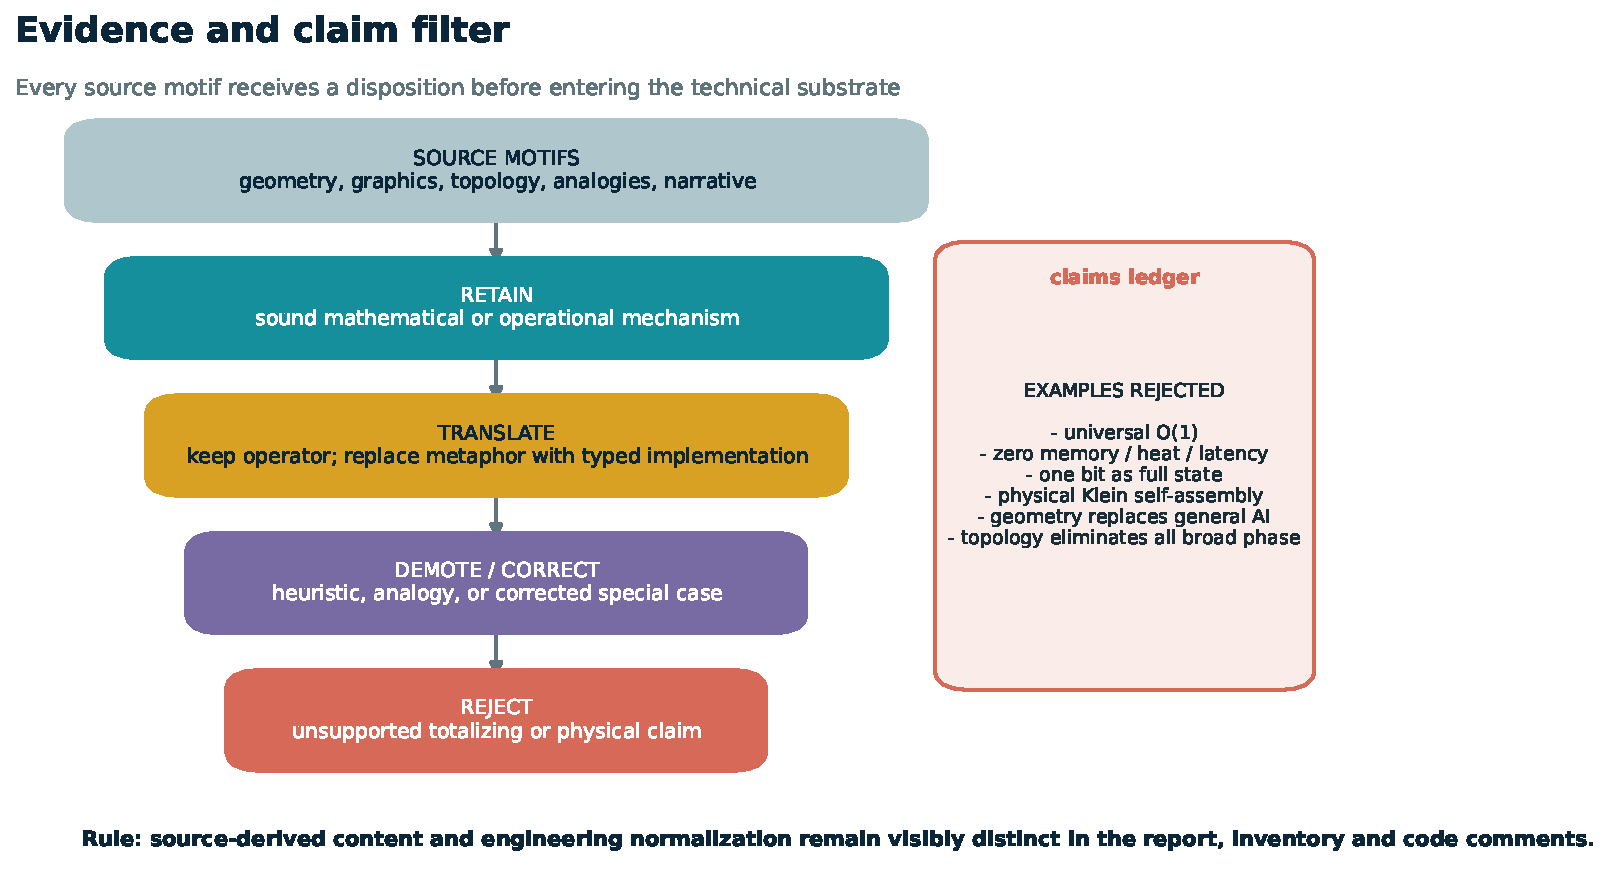
\includegraphics[width=0.96\textwidth]{evidence_filter.pdf}
\caption{The report preserves useful operators while correcting or rejecting unsupported claims.}
\end{figure}

Each item is marked \statusretain, \statustranslate, \statusdemote / \statuscorrect, or \statusreject. Source-derived statements and engineering normalization are kept separate throughout the inventory and code comments.

\chapter{Method and source architecture}
\section{Corpus handling}
Nine PDFs were read as design records. Repeated dialogue bundles were deduplicated: S2, S8 and S9 share much of the D/B/phi-to-R thread, so repeated text is not counted as independent validation. S6 and S5 are given the greatest interpretive weight because they explicitly impose feasibility, type-safety, calibration and falsifiability constraints on earlier material.

\begingroup
\footnotesize
\setlength{\tabcolsep}{2.5pt}
\renewcommand{\arraystretch}{1.08}
\begin{longtable}{@{}L{0.055\textwidth}L{0.19\textwidth}L{0.34\textwidth}L{0.37\textwidth}@{}}
\caption{Source corpus and role in the extraction. File names are concise aliases; source IDs and page ranges are authoritative within this package.}\label{tab:sources}\\
\toprule Ref & Short name & File alias & Role \\ \midrule
\endfirsthead
\multicolumn{4}{l}{\small\itshape Table \ref{tab:sources} continued}\\
\toprule Ref & Short name & File alias & Role \\ \midrule
\endhead
\bottomrule\endlastfoot
S1 & \path{NUM19}\par{\tiny 30 pages} & \path{numeric-fractal-dialogue.pdf} & Numeric, phonetic, binary, triangle, Pascal/Sierpinski, graphics and topology motif chain. \\
\addlinespace[3pt]
S2 & \path{AUTHOR_DIALOGUE}\par{\tiny 52 pages} & \path{author-dialogue-bundle-[identifiers-omitted].pdf} & Extended dialogue bundle; duplicates the D/B/phi-to-R thread and adds AR, cognition, networking, and narrative extrapolations. \\
\addlinespace[3pt]
S3 & \path{KC_GRAPHICS}\par{\tiny 10 pages} & \path{kc-vector-graphics.pdf} & Graphics adapter: log-polar mapping, SDF/CSG, phasor-style coverage, 1-bit temporal/spatial modulation, chromatic offsets, prepress. \\
\addlinespace[3pt]
S4 & \path{BEN_BURGER}\par{\tiny 19 pages} & \path{ben-burger-zero-index-dialogue.pdf} & Zero-based indexing, split-oval/torque wave motif, overlapping semicircles, shared-domain interpretation. \\
\addlinespace[3pt]
S5 & \path{WAVEGUIDE}\par{\tiny 12 pages} & \path{spherical-throughput-waveguide.pdf} & Bounded optofluidic hardware translation, B.C.E. logic, metrics, fabrication and kill criteria. \\
\addlinespace[3pt]
S6 & \path{CHRONO_SYNTHESIS}\par{\tiny 12 pages} & \path{chronological-spherical-substrate-synthesis.pdf} & Mature internal synthesis: query-first event calculus, local spherical support, compatibility, lineage, feasibility discipline. \\
\addlinespace[3pt]
S7 & \path{HOLLOWLAND}\par{\tiny 36 pages} & \path{hollowland-double-vacuum.pdf} & Double-vacuum, phase sheets, analytic cones, hourglass routing, procedural grammar, kinematic calculus and highly speculative extensions. \\
\addlinespace[3pt]
S8 & \path{GEORGE_BUNDLE}\par{\tiny 42 pages} & \path{george-dialogue-bundle.pdf} & Substantially overlapping D/B/phi-to-R dialogue bundle; later pages add perception, storage and related extrapolations. \\
\addlinespace[3pt]
S9 & \path{D_TO_PH}\par{\tiny 34 pages} & \path{d-to-ph-glyph-topology.pdf} & Core glyph morph, parity hinge, log-polar/L-system, SDF-global hinge and topology motif thread. \\
\addlinespace[3pt]
\end{longtable}
\endgroup


\section{Extraction dimensions}
Every candidate mechanism was tested against five questions:
\begin{enumerate}
\item \textbf{Geometry:} Is there a definable curve, field, support, transform or invariant?
\item \textbf{Topology:} Is there an explicit gluing, orientation, sheet or routing operation?
\item \textbf{Information architecture:} What state, schema, query, event and provenance are required?
\item \textbf{Game technology:} Can the mechanism be expressed as a component, system or adapter?
\item \textbf{Evidence boundary:} Is the statement exact, heuristic, speculative or contradicted by ordinary engineering constraints?
\end{enumerate}

\section{Deduplication and personal-data discipline}
The source corpus includes filenames and dialogue text containing personal identifiers. They are not necessary to the geometrical synthesis and are omitted. The package does not redistribute the original PDFs. Source traceability is by S1--S9, page ranges and descriptive filenames only.

\chapter{Numeric and fractal seeds}
\section{Radix carry thresholds}
\statusretain\quad In base $b$, a new digit is required at $b^k$. This is an exact positional-number fact and provides a useful scale/level boundary:
\[
\operatorname{digits}_b(n)=\begin{cases}1,&n=0,\\ \lfloor\log_b n\rfloor+1,&n>0.\end{cases}
\]
The source begins with binary transitions $1\to10$, $11\to100$, and the decimal transition $9\to10$ (S1, pp. 1--4). UGTS-0 uses radix powers as compact hierarchy thresholds, never as proof that geometry is inherently binary.

\section{Zero-based offset semantics}
\statusretain\quad S4 correctly distinguishes an index from an ordinal: index 35 is the 36th position. The arithmetic $21+7+7=35$ is unchanged. The implementation exposes \code{zero\_based\_ordinal(35) == 36} to prevent the narrative ``shift'' from becoming an off-by-one ambiguity.

\section{Active bits and the triangle seed}
\statustranslate\quad $19=10011_2$ has active positions $\{4,1,0\}$ and Hamming weight three. The source maps those three active positions to three Dutch syllables and then to a triangle (S1, pp. 3--7). The technically valid core is popcount and a chosen simplex embedding. The syllable equality is a mnemonic; it is not a general number-language code.

\section{Pascal parity and Sierpinski}
\statusretain\quad Binomial parity is a deterministic fractal generator:
\[
\binom{n}{k}\equiv1\pmod2 \quad\Longleftrightarrow\quad k\ \&\ \neg n=0.
\]
This follows from Lucas-style bit containment. The source's visual connection is valid, with one correction: zero-based rows $2^m-1$ are all odd; generic rows $2^m$ are not. The package contains \code{pascal\_entry\_is\_odd} and a PBM generator.

\begin{figure}[H]
\centering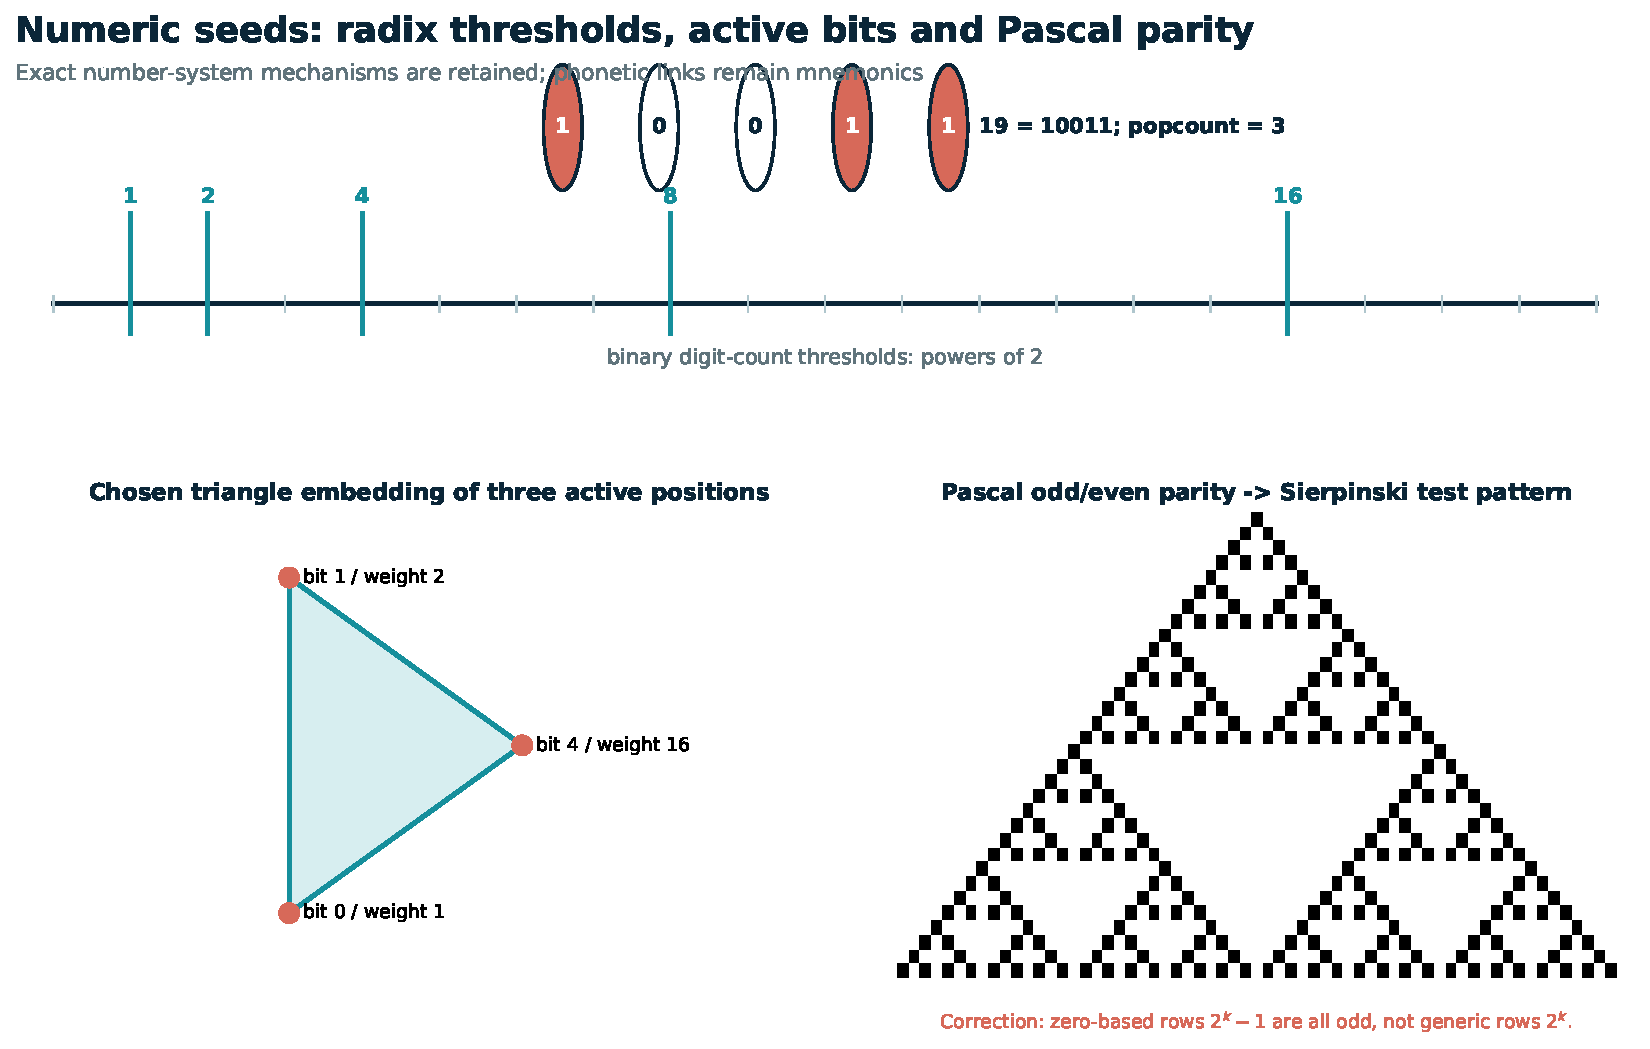
\includegraphics[width=\textwidth]{numeric_fractal.pdf}
\caption{Exact numeric mechanisms retained from S1 and S4.}
\end{figure}

\section{Golden-angle sampling and strange loops}
\statustranslate\quad Vogel/golden-angle points are useful as a low-regularity sample schedule. They can reduce obvious repetition but do not guarantee zero aliasing or zero cost. \statusdemote\quad Lemniscates and Escher loops are retained only as recursion motifs. In UGTS-0 recursion is finite, budgeted and cycle-detectable through \code{FiniteGrammar}; no self-creating physical substrate is asserted.

\chapter{Glyph geometry and kinematic tricks}
\section{Loop-plus-stem decomposition}
S2, S8 and S9 repeatedly decompose a selected glyph form into a vertical stem plus one or more closed arcs. This depends on the font and therefore becomes a design convention, not a theorem about letters.

\section{Cut/unroll D or B into R}
\statusretain\quad The clearest individual geometrical trick is a boundary-graph edit:
\begin{enumerate}
\item Keep the vertical stem and upper loop.
\item Cut the lower closed arc at its anchor.
\item Release one endpoint.
\item Continuously interpolate the released arc/control points toward a diagonal segment.
\end{enumerate}
This is directly implementable in vector paths, spline control meshes or implicit transition fields. The code provides \code{loop\_to\_r\_morph(alpha)}.

\begin{figure}[H]
\centering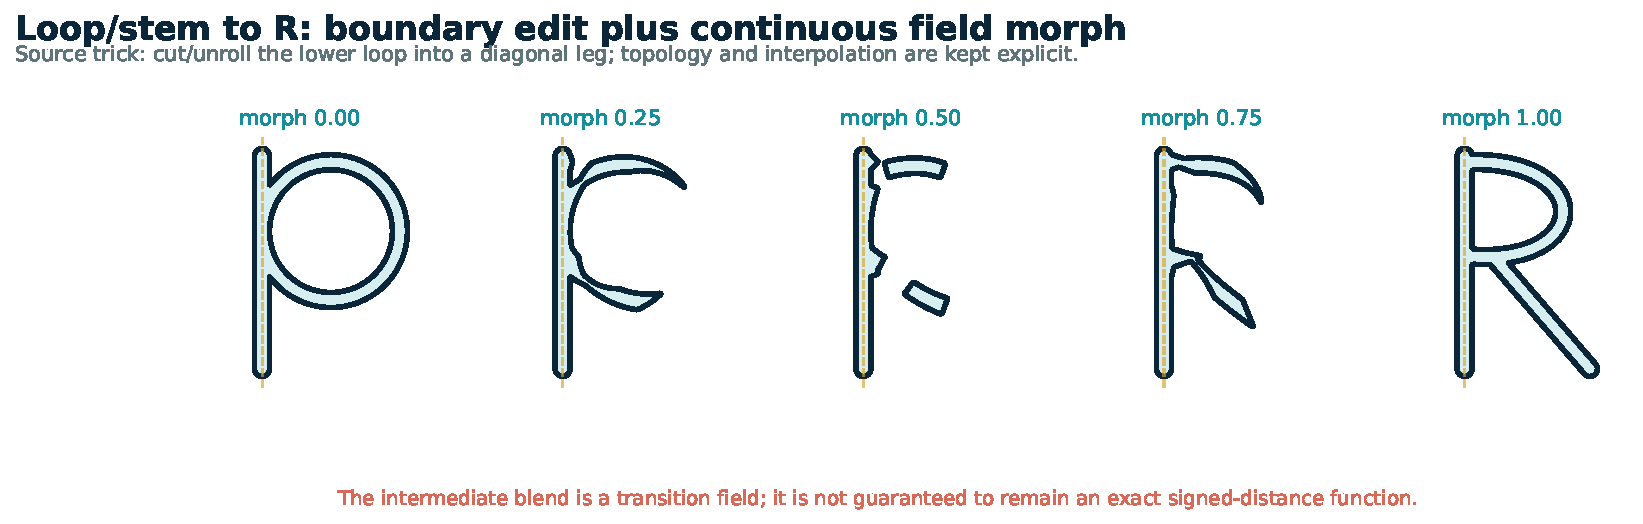
\includegraphics[width=\textwidth]{glyph_morph.pdf}
\caption{The D/B/phi-to-R motif normalized as a path/field morph.}
\end{figure}

\section{Torque axis, time and phase}
\statustranslate\quad The source calls the stem a torque axis $T$ and uses $\Delta T$ and $\Delta\phi$ for motion. UGTS-0 separates the overloaded symbols:
\begin{itemize}
\item continuous time $t$ and time increment $\Delta t$,
\item orientation/rotation parameter $\theta$,
\item physical torque $\tau$ only when a mechanical model is supplied,
\item phase $\phi\in S^1$ and phase rate $\dot\phi$.
\end{itemize}
This type separation prevents a triangle, torque, time step and transformation from silently sharing one symbol.

\section{One-bit hinge and global morph}
\statusretain\quad A bit may select closed/open, route A/B, admitted/rejected or stale/fresh according to a declared schema. \statustranslate\quad ``The hinge is everywhere'' becomes a global transition field or state patch evaluated at all queried points. A linear field blend is useful for visualization but intermediate fields need not be exact SDFs, and a topology change still requires an explicit gluing/transition rule.

\section{Split oval, opposing arches and overlap lens}
S4 contributes two usable constructions. First, a split oval under antisymmetric displacement becomes two curve branches around a fixed node. The source's 1:1 amplitude is a symmetric example, not universal warped-disk physics. Second, two overlapping semicircles create a measurable lens region:
\[
A_{\text{lens}}=2r^2\cos^{-1}\!\left(\frac d{2r}\right)-\frac d2\sqrt{4r^2-d^2}.
\]
The lens can represent geometric intersection, a tolerance buffer, a blend zone or shared information $A\cap B$; its semantics must be specified by the application.

\chapter{Implicit geometry and analytic events}
\section{Implicit fields and sign convention}
\statusretain\quad A field $f:\mathbb R^n\to\mathbb R$ uses $f=0$ as boundary, $f<0$ as interior and $f>0$ as exterior. Exact signed-distance status is reserved for valid primitives and distance-preserving transforms. A generic implicit field is not automatically an exact SDF.

\section{Constructive solid geometry}
The KC graphics document supplies the standard operators:
\[
 f_{A\cup B}=\min(f_A,f_B),\qquad
 f_{A\cap B}=\max(f_A,f_B),\qquad
 f_{A\setminus B}=\max(f_A,-f_B).
\]
UGTS-0 implements these plus a documented smooth union and a non-distance-preserving morph field.

\section{The zero surface becomes an event relation}
This is the most important correction in the corpus. Earlier material tends to treat $f=0$ as a graphics boundary to sample or march through. S6 instead promotes it to an event relation $R_j(q)=0$. The system solves the crossing time and invokes transition semantics. Rendering can still sample the field, but the authoritative state change is an event.

\section{Closed-form and numerical solvers}
\statusretain\quad For a line relation $n\cdot x=c$ and a quadratic trajectory
\[
x(t)=p_0+v_0\Delta t+\tfrac12a\Delta t^2,
\]
the crossing is a quadratic root. For a circle and linear trajectory, the crossing is also quadratic. \statusreject\quad Arbitrary SDF/trajectory pairs do not have universal exact non-iterative roots. UGTS-0 falls back to sampled bracketing and bisection for a declared generic field.

\begin{riskbox}
Tangencies, coincident surfaces, multiple roots, long horizons, singular log coordinates and rank changes are part of the engineering problem. Solvers must return tolerance, confidence/status and reason codes rather than pretending every event is exact.
\end{riskbox}

\chapter{Local supports: cone, sphere, shell and hourglass}
\section{Cone as analytic relevance}
\statusretain\quad A cone is a local admission domain: field of view, directional influence, collision scope, memory-retrieval scope or coupler acceptance. In 2D the package uses radius, center angle, half-width and time interval. It need not be drawn.

\section{Spherical means local radial-angular chart}
S5 and S6 explicitly state that spherical does not require a global spherical world. It means a local chart around a sensor or coupler containing angular support, radial reach, orientation, uncertainty and field of view. The global substrate may remain Euclidean, graph-backed, projective or hybrid.

\section{Nested shells}
\statustranslate\quad Concentric shell intervals can organize multiresolution range or relevance. They are useful as a local index but are not required everywhere. A shell hierarchy is orthogonal to entity identity and does not replace a generic spatial index for unsupported scenes.

\section{Quad hourglass and invariant axis}
\statustranslate\quad The source's four chambers meeting at a pinch become a finite routing table. The pinch is an event locus, not a physical singularity. An invariant/eigen-axis is retained as a stable mode/direction under a transformation; eigenvalue rhetoric is not used as a magical binary switch.

\chapter{Topology as explicit gluing}
\section{Phase sheets and double vacuum}
\statusretain\quad The strongest topological/information concept is that two states may share the same coordinate yet fail to interact. The ``second vacuum'' is absence of coupling, not deeper emptiness. The compatibility test can include sheet, phase, orientation, branch, tags, policy and lineage.

\begin{examplebox}
At $t=2$, entities A and B can both occupy $(0,0.25)$. If A is on sheet 0 with phase 0 and B is on sheet 1 with phase $\pi$, \code{can\_couple} returns false with \code{sheet\_mismatch} and \code{phase\_mismatch}. Co-location is necessary but not sufficient.
\end{examplebox}

\section{Mobius and Klein quotient maps}
\statusretain\quad A Mobius band can be implemented as a rectangle quotient $(0,y)\sim(w,-y)$, which flips orientation after one wrap. \statustranslate\quad A Klein-bottle motif becomes an explicit two-axis quotient where one wrap flips orientation/sheet and the other closes periodically. It is a software coordinate/gluing map, not a claim that matter passes through itself physically.

\section{Topological portals}
A portal is specified by:
\begin{itemize}
\item entry event surface and admission support,
\item exit coordinate transform,
\item orientation and sheet map,
\item phase/branch policy,
\item lineage event and uncertainty.
\end{itemize}
This is sufficient for non-orientable game spaces without requiring a physically embedded Klein bottle.

\begin{figure}[H]
\centering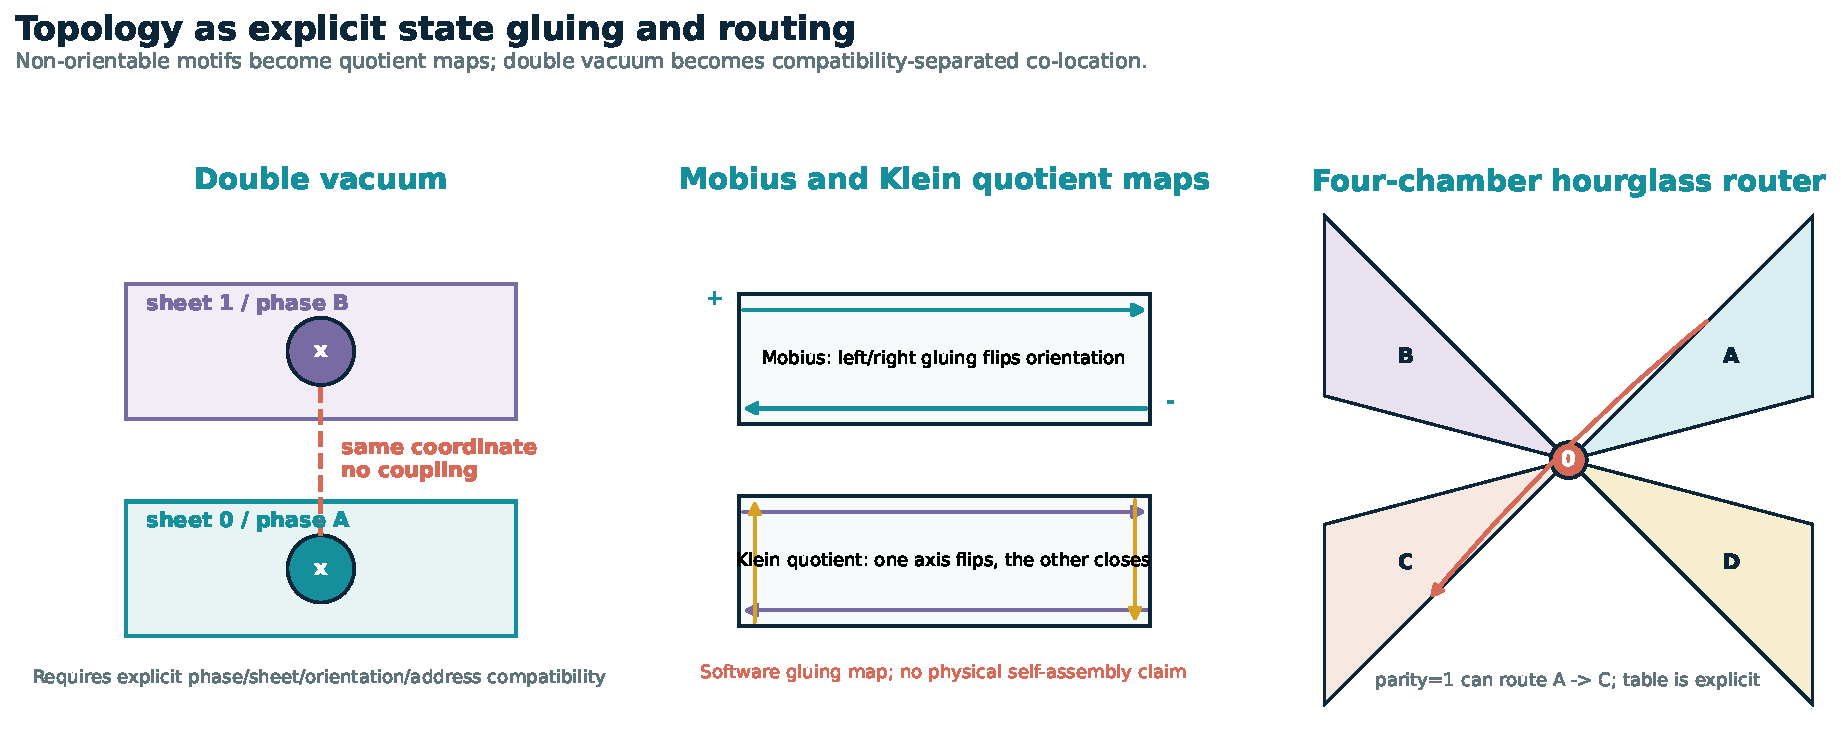
\includegraphics[width=\textwidth]{topology_maps.pdf}
\caption{Double vacuum, quotient gluing and hourglass routing after normalization.}
\end{figure}

\section{Inside/outside is schema-bound}
The sign of an implicit field, the parity bit and the orientation bit are separate typed values. ``Inside'' cannot be inferred from parity without a schema. This mirrors the corpus's COBOL packed-decimal lesson: raw bits are meaningless without layout metadata.

\chapter{Information architecture formalism}
\section{Typed state manifold}
A compact reference state is
\[
q_e(t)=\bigl(x_e(t),\ t,\ \phi_e(t),\ s_e(t),\ o_e(t),\ a_e,\ b_e(t),\ u_e(t)\bigr),
\]
where $x$ is position, $\phi$ phase, $s$ sheet, $o\in\{-1,+1\}$ orientation, $a$ lineage address, $b$ branch and $u$ uncertainty. A corresponding abstract space is
\[
Q=P^n\times\mathbb R_{time}\times S^1_{phase}\times S_{sheet}\times O_{orientation}\times A_{address}\times B_{branch}\times U.
\]

\section{World definition}
The world is not only geometry:
\[
W=(G,R,T,I,L),
\]
with finite grammar $G$, relation family $R$, transition family $T$, invariants $I$, and external event log $L$.

\section{Support, compatibility, event and transition}
For relation $j$ and support $\alpha$:
\[
R_j(q;\theta_j)=0,\qquad C_\alpha(q,t)\le0,\qquad \chi(e,j,t)\in\{0,1\}.
\]
The next event is
\[
t^*=\min\{t>t_0:R_j(q_e(t))=0,\ C_\alpha(q_e(t),t)\le0,\ \chi(e,j,t)=1\}.
\]
The transition produces a patch and event record:
\[
q_e(t^{*+})=T_j(q_e(t^{*-}),\text{context}).
\]

\begin{figure}[H]
\centering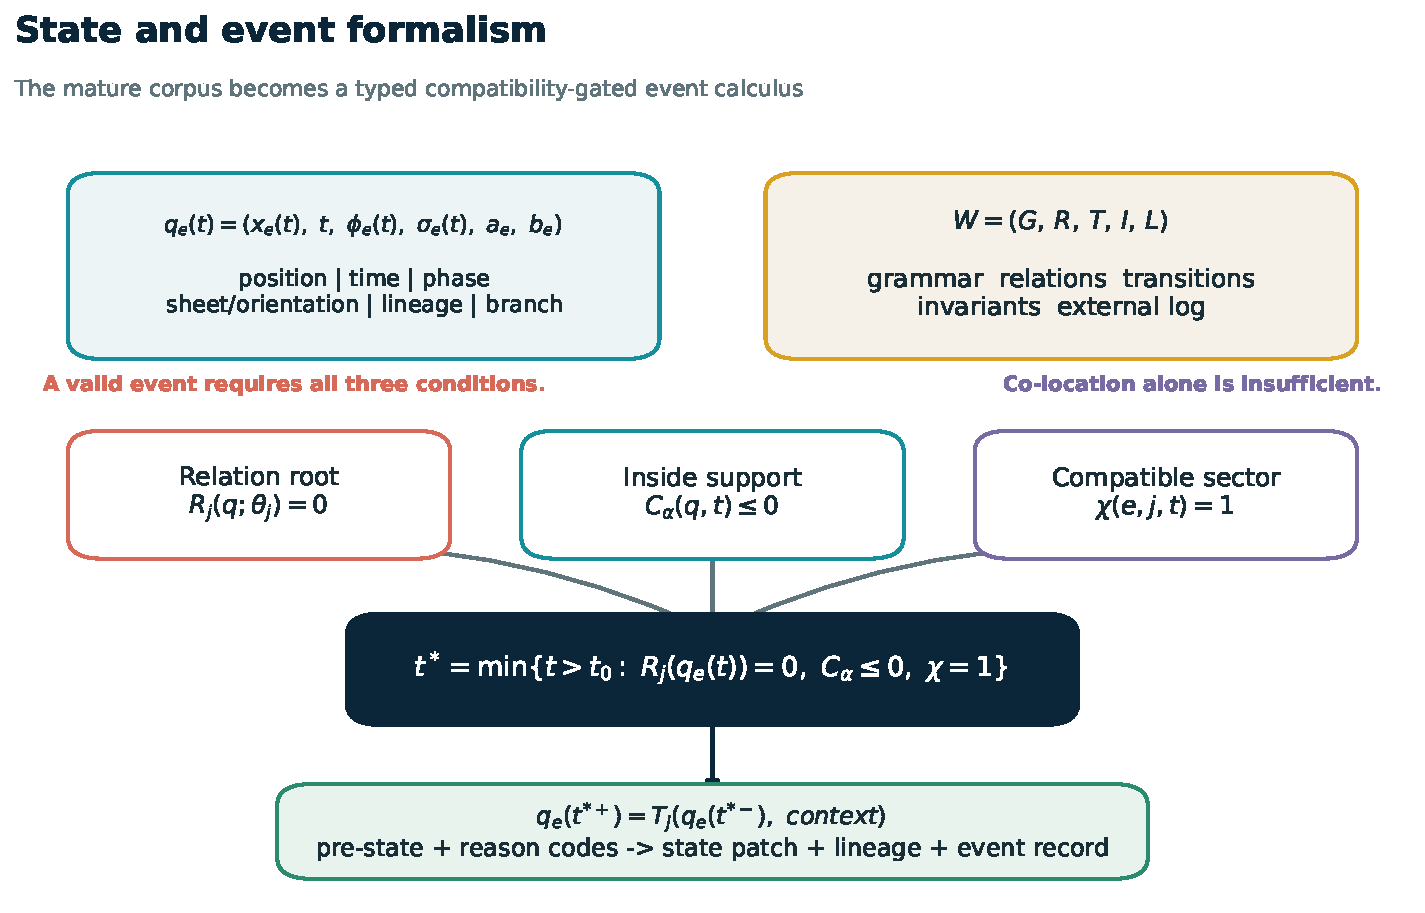
\includegraphics[width=\textwidth]{state_event_formalism.pdf}
\caption{The formal event condition requires relation, support and compatibility.}
\end{figure}

\section{Reason codes and confidence}
A boolean is insufficient for engineering. Compatibility returns reason codes such as sheet mismatch, phase mismatch, missing tag or policy rejection. An event record contains pre/post state, solver family, crossing direction, relation residual, confidence, lineage and metadata.

\chapter{Finite grammar, identity and memory}
\section{Finite grammar}
\statusretain\quad L-system and shape-grammar language is useful only after depth and symbol budgets are explicit. The implementation refuses expansion beyond \code{max\_depth} or \code{max\_symbols}; unknown variables are inert rather than magical.

\section{Lineage address}
Coordinates are not identity. An entity keeps a stable ID plus transition ancestry. Portals, branch changes, splits and merges must append lineage records or create explicit parent/merge references. This allows identity reconstruction even after co-location or coordinate reuse.

\section{External event log}
Closed deterministic dynamics may be recomputed from parameters, but exogenous novelty cannot. The irreducible log records inputs, branch choices, calibration changes, policy decisions and uncertain solver outcomes. Therefore the substrate can reduce frame storage in restricted cases but cannot be zero-memory.

\section{Schema-bound packed data}
S2/S8/S9 discuss COBOL COMP-3 and copybooks. The useful lesson is architectural: a byte stream without layout is not self-describing. UGTS-0 versions world schemas, event schemas, LUT dimensions, sign conventions and parity meanings.

\chapter{Query-first runtime and complexity}
\section{Minimum API}
The six minimum queries are:
\begin{enumerate}
\item \code{state\_at(entity,t)}
\item \code{next\_event(entity,t0,t1)}
\item \code{events\_in\_support(support,t0,t1)}
\item \code{can\_couple(a,b,t)}
\item transition application / event processing
\item \code{reconstruct\_identity(entity)}
\end{enumerate}

\section{Precise meaning of horizon skipping}
For a fixed closed expression, \code{state\_at(t)} can be independent of the number of skipped simulation frames. This is not universal O(1): expression size, grammar depth, branch history and transcendental evaluation still cost resources. \code{next\_event} is dominated by candidate filtering, root solving and branch resolution.

\section{Success criterion}
The architecture wins only if
\[
\operatorname{cost}(\text{support}+\text{compatibility}+\text{event solve})
<\operatorname{cost}(\text{explicit materialization avoided})
\]
for the target relation family and error boundary. Poor compatibility predicates turn cone queries into broad scans; dense events or grammar growth can erase any advantage.

\chapter{Game-technology integration}
\section{Hybrid engine structure}
A practical game engine does not need to abandon conventional systems. The authoritative UGTS state can coexist with meshes, rigid bodies, audio, animation, editor tooling and rasterization.

\begin{figure}[H]
\centering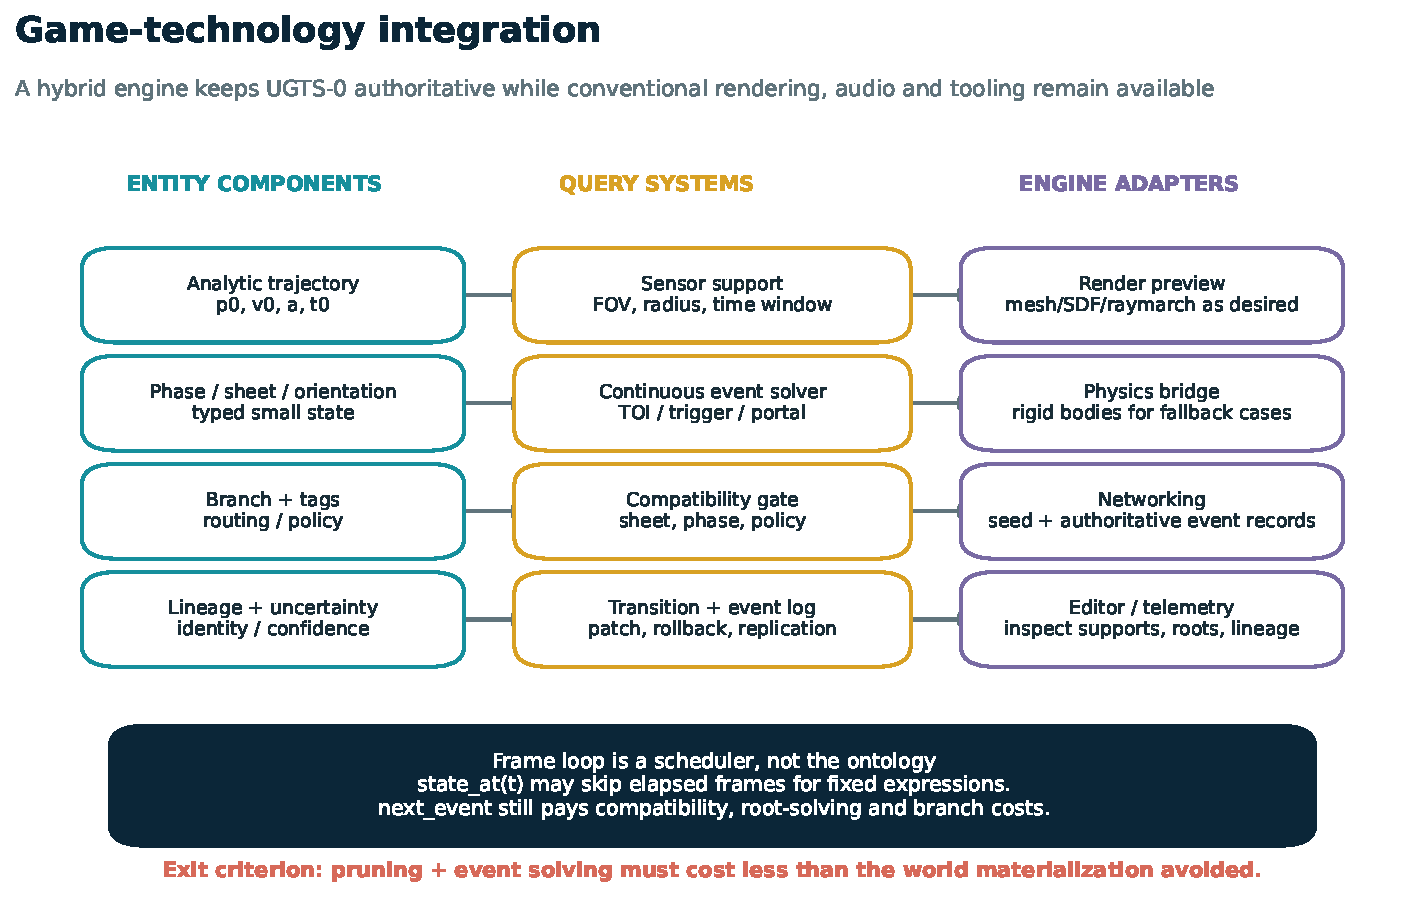
\includegraphics[width=\textwidth]{game_engine_stack.pdf}
\caption{Component/system mapping for Unity, Godot or an ECS runtime.}
\end{figure}

\section{Components}
\begin{description}[style=nextline]
\item[Analytic motion component] Coefficients for linear or quadratic trajectory plus start time.
\item[Phase/sheet/orientation component] Small typed state, never collapsed into one unnamed bit.
\item[Support component] Local FOV, radial range and time window.
\item[Relation component] Line, circle or generic implicit event surface.
\item[Transition component] Sheet/orientation/phase/branch/tag patch with lineage label.
\item[Event-log component] Authoritative event records for rollback and replay.
\end{description}

\section{Continuous collision and portals}
For supported relations, time of impact is solved analytically. Unsupported cases can fall back to a conventional physics engine or numerical method. A portal is just an event surface plus explicit exit map and state patch, making Mobius/Klein/hourglass effects deterministic and inspectable.

\section{Networking}
Seed/parameter replication plus authoritative event records can reduce frame replication for stable closed dynamics. Cross-platform floating-point differences, nondeterministic branches and exogenous inputs still require synchronization, schema versions and correction snapshots.

\section{Adapters supplied}
The package includes minimal Unity C\# and Godot GDScript adapters. They demonstrate \code{state\_at} and a line-crossing query without claiming full engine integration.

\chapter{Optional graphics projection}
\section{Log-polar chart}
\statusretain\quad The local map is
\[
\rho=\ln(r/r_0),\qquad\theta=\operatorname{atan2}(y,x).
\]
Scaling in real space becomes translation in $\rho$. The origin remains singular, so UGTS-0 uses an explicit epsilon/core flag; the logarithm does not remove the singularity.

\section{One-bit log-polar LUT}
A compact bitset marks active $(\rho,\theta)$ sectors. It is a mask for admission or projection work, not complete world state. LUT dimensions, range, origin convention and bit meaning are schema fields.

\section{Phasor edge accumulation}
\statustranslate\quad The source calls its subpixel vectors ``Feynman vectors.'' UGTS-0 normalizes this to ordinary complex phasors whose phase follows local field-gradient orientation and whose magnitude follows coverage. This can be used for oriented supersampling; no quantum path-integral claim is made.

\section{One-bit jitter and temporal modulation}
\statusretain\quad A static projection can use deterministic stochastic thresholds. \statustranslate\quad A display can use pulse-density/sigma-delta bitstreams to approximate intensity over time. These are optional output encodings and require hardware calibration.

\section{Chromatic and prepress transforms}
A real-space magnification $r\mapsto sr$ becomes $\rho\mapsto\rho+\ln s$, so channel-specific chromatic scale can be expressed as a log-radius offset. It is cheap, not free. The prepress adapter maps channels to CMYK, uses log-radius-dependent screening and must compensate dot gain and moire risk.

\begin{figure}[H]
\centering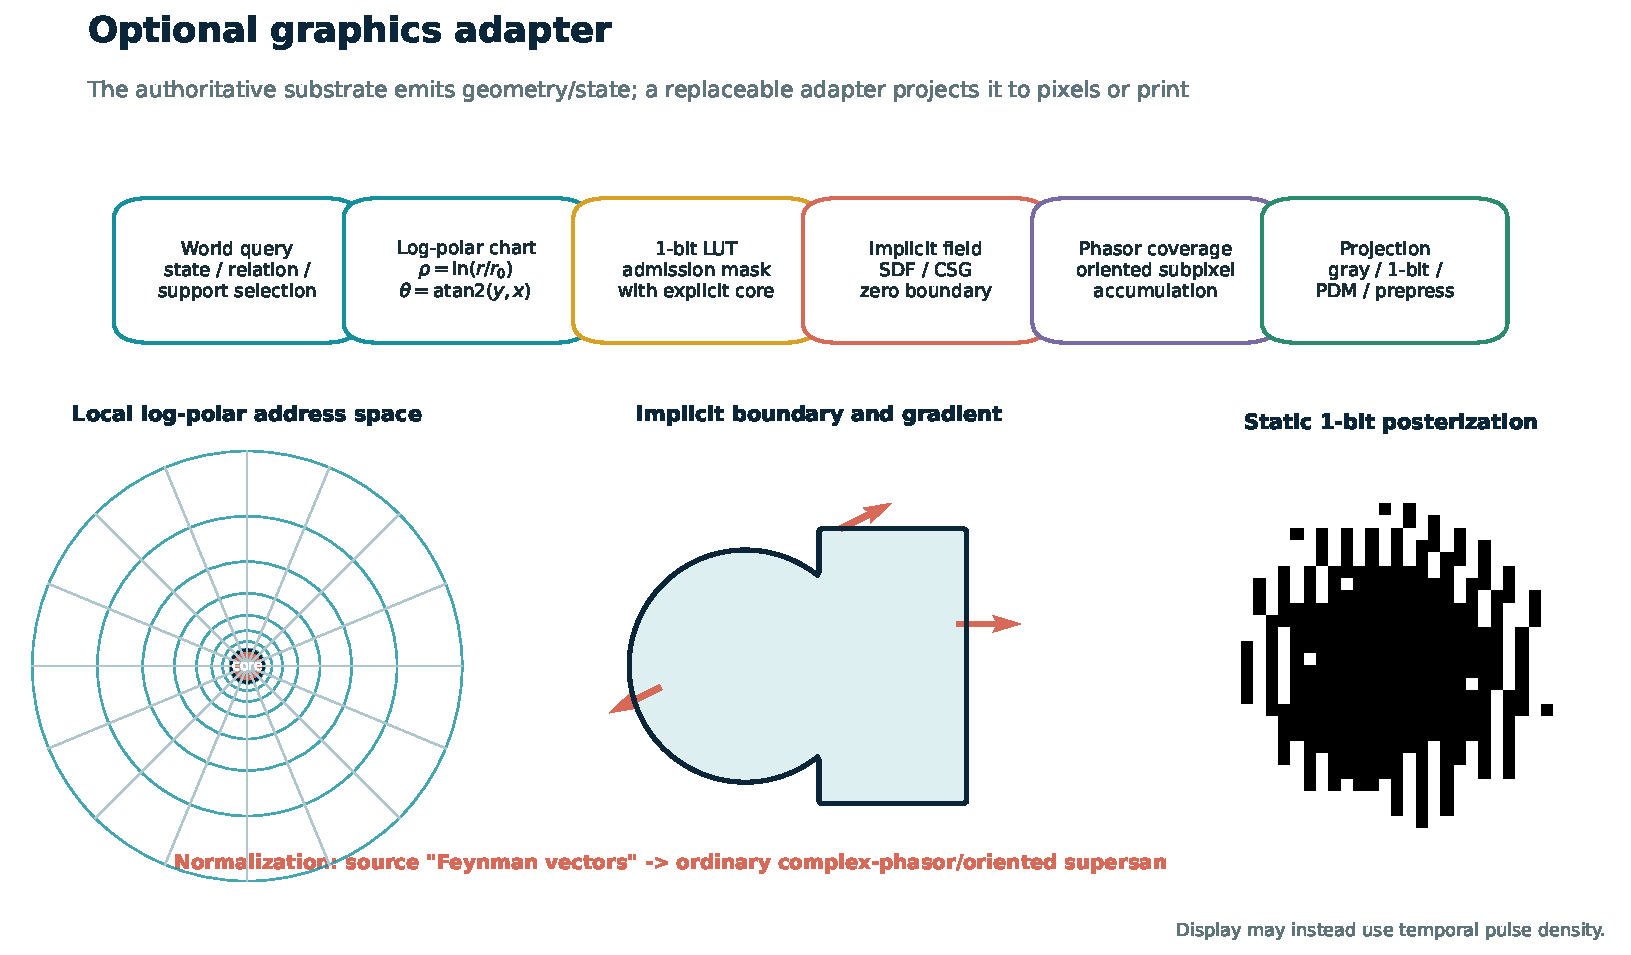
\includegraphics[width=\textwidth]{graphics_adapter.pdf}
\caption{The KC graphics material becomes a replaceable projection pipeline.}
\end{figure}

\chapter{Bounded Compatibility Event hardware endpoint}
\section{Canonical signal path}
S5 gives the best-defined physical translation:
\[
\text{local support}\rightarrow\text{liquid-controlled coupling}\rightarrow
\text{compatible mode}\rightarrow\text{measured guard}\rightarrow\text{verified output}.
\]
A local radial-angular optical field is focused or phase-shaped by a liquid region, coupled into selected guided modes, filtered by wavelength/polarization/mode/phase compatibility, and declared an event only at a measured guard crossing.

\section{Type safety across physics}
Maxwell governs the optical field; Young--Laplace/fluid mechanics governs the meniscus; coupled-mode theory governs guided amplitudes; digital event logic decides when a result is declared. A Klein motif may describe routing only after ports, orientation map and transfer matrix are specified.

\section{Narrow parity role}
The parity bit can mark route, admission, freshness or latch state. Detector amplitudes, thresholds, confidence, uncertainty, calibration and lineage remain separate. The reference controller detects a rising/falling threshold crossing only after support and compatibility are true.

\begin{figure}[H]
\centering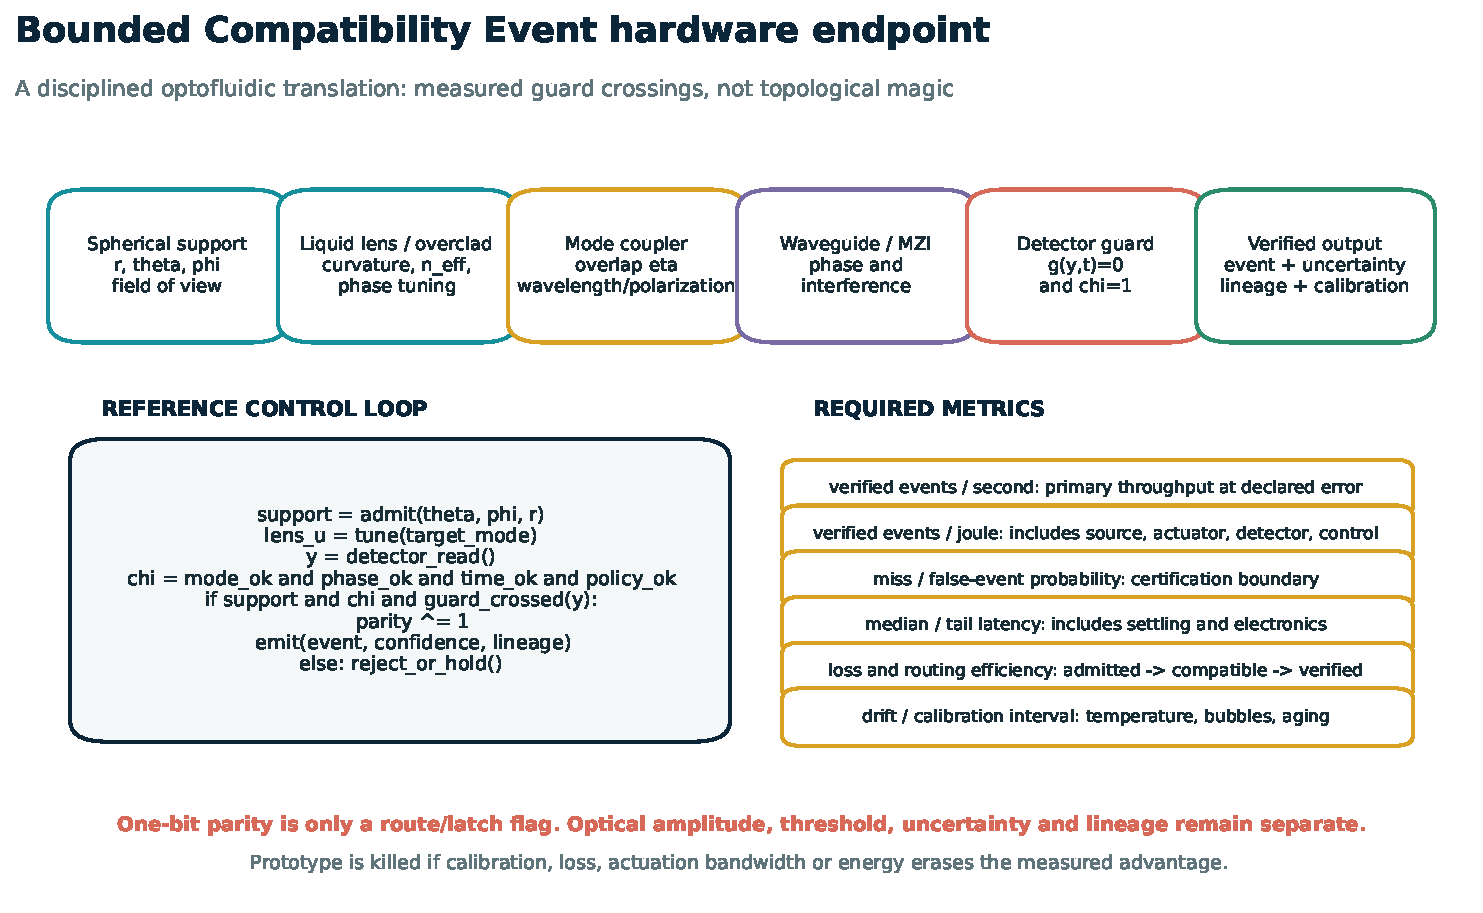
\includegraphics[width=\textwidth]{bce_hardware.pdf}
\caption{B.C.E. signal path, control loop and required metrics.}
\end{figure}

\section{Hollowlens-0}
The source proposes one scanned input, one tunable liquid coupler, a $2\times2$ interferometric waveguide, balanced detectors and an FPGA/MCU sidecar. Success requires preregistered wavelength, power, support, compatible modes, thresholds, uncertainty, energy boundary, calibration interval and matched electronic baseline.

\section{Kill criteria}
The prototype is stopped or simplified if optical loss, liquid instability, slow actuation, mode crosstalk, calibration drift, event ambiguity, packaging failure or sidecar dominance removes the energy/accuracy advantage.

\chapter{Reference implementation}
\section{Package structure}
\begin{lstlisting}[language={},caption={Delivered package layout}]
README.md                  technical entry point
specs/                     source map, 69 concepts, claims, schemas
src/ugts/                  dependency-free Python reference runtime
tests/test_ugts.py         executable verification
examples/                  world, topology, graphics, fractal, B.C.E. demos
shaders/ugts_preview.frag  optional GLSL projection
adapters/unity/            minimal C# game adapter
adapters/godot/            minimal GDScript game adapter
diagrams/                  report figures
source_notes/              per-PDF extraction notes
\end{lstlisting}

\section{Core modules}
\begin{longtable}{@{}p{0.22\textwidth}p{0.72\textwidth}@{}}
\toprule Module & Responsibility \\ \midrule\endhead
\code{state.py} & Typed entity state, state patches, lineage and event records.\\
\code{trajectory.py} & Closed-form linear and quadratic motion.\\
\code{support.py} & Local radial-angular and time admission.\\
\code{compatibility.py} & Sheet, orientation, phase, branch, tags and lineage gating.\\
\code{events.py} & Analytic line/circle roots and bracketed generic-field roots.\\
\code{transition.py} & Pure schema-bound state patches.\\
\code{world.py} & Query API, transition processing, double-vacuum coupling and event log.\\
\code{geometry.py} & Implicit primitives, CSG, morph, gradient and overlap lens.\\
\code{topology.py} & Mobius/Klein quotient maps, portals and hourglass routing.\\
\code{logpolar.py} & Explicit-core transform and compact bit LUT.\\
\code{numeric.py} & Radix, Hamming, Pascal parity and golden-angle samples.\\
\code{glyphs.py} & Loop/stem and loop-to-R transition fields.\\
\code{grammar.py} & Finite budgeted grammar and small shape compiler.\\
\code{render.py} & Optional CPU projection, posterization and PDM.\\
\code{bce.py} & Measured compatibility/guard controller.\\
\code{io.py} & JSON world loader and event-log serialization.\\
\bottomrule
\end{longtable}

\section{World query example}
\begin{lstlisting}[language=Python,caption={Minimal query-first use}]
from ugts import load_world

world = load_world("specs/example_world.json")
state = world.state_at("traveler_A", 1.25)
candidate = world.next_event("traveler_A", 0.0, 5.0)
record = world.process_next_event("traveler_A", 0.0, 5.0)

coupling = world.can_couple(
    "traveler_A", "co_located_B", 2.0,
    max_distance=1e-9,
    phase_tolerance=0.2,
    require_same_sheet=True,
    require_same_orientation=True,
)
\end{lstlisting}

\section{Event solver behavior}
Line surfaces support linear and quadratic trajectories. Circle surfaces currently support analytic roots for linear trajectories. Generic fields use a sampled sign-change search followed by bisection. The solver excludes the current instant by an epsilon, applies support and compatibility, then sorts candidate events by time and rule ID.

\section{Topological map behavior}
\begin{lstlisting}[language=Python,caption={Explicit quotient maps}]
from ugts import MobiusBand, KleinBottleQuotient, Vec2

mobius = MobiusBand(width=4.0, height=2.0)
print(mobius.map(Vec2(4.5, 0.25)))
# x wraps to 0.5; y and orientation flip

klein = KleinBottleQuotient(width=4.0, height=2.0)
print(klein.map(Vec2(4.5, 0.25)))
# orientation flips and sheet toggles
\end{lstlisting}

\chapter{Verification and test results}
\section{Executable tests}
The package includes seventeen tests across numeric seeds, implicit geometry, event solving, transitions, double-vacuum coupling, quotient maps, log-polar roundtrip, bit-LUT storage, rendering, grammar budgets, B.C.E. and JSON I/O.

\lstinputlisting[language={},caption={Test run captured during package construction}]{test_results.txt}

\section{What the tests establish}
The tests establish internal consistency of the bounded implementation. They do not validate the corpus's external performance, physical hardware throughput or universal claims. In particular, they demonstrate that:
\begin{itemize}
\item the traveler crosses $x=0$ at $t=2$ and receives the expected sheet/orientation/branch patch;
\item co-located incompatible states do not couple;
\item Mobius and Klein quotient maps apply declared orientation/sheet changes;
\item Pascal row 7 is all odd while row 8 is not;
\item log-polar conversion requires an explicit core chart;
\item the one-bit LUT uses the expected compact storage;
\item the B.C.E. bit toggles only after a valid measured crossing.
\end{itemize}

\chapter{Prototype program and falsification}
\begin{figure}[H]
\centering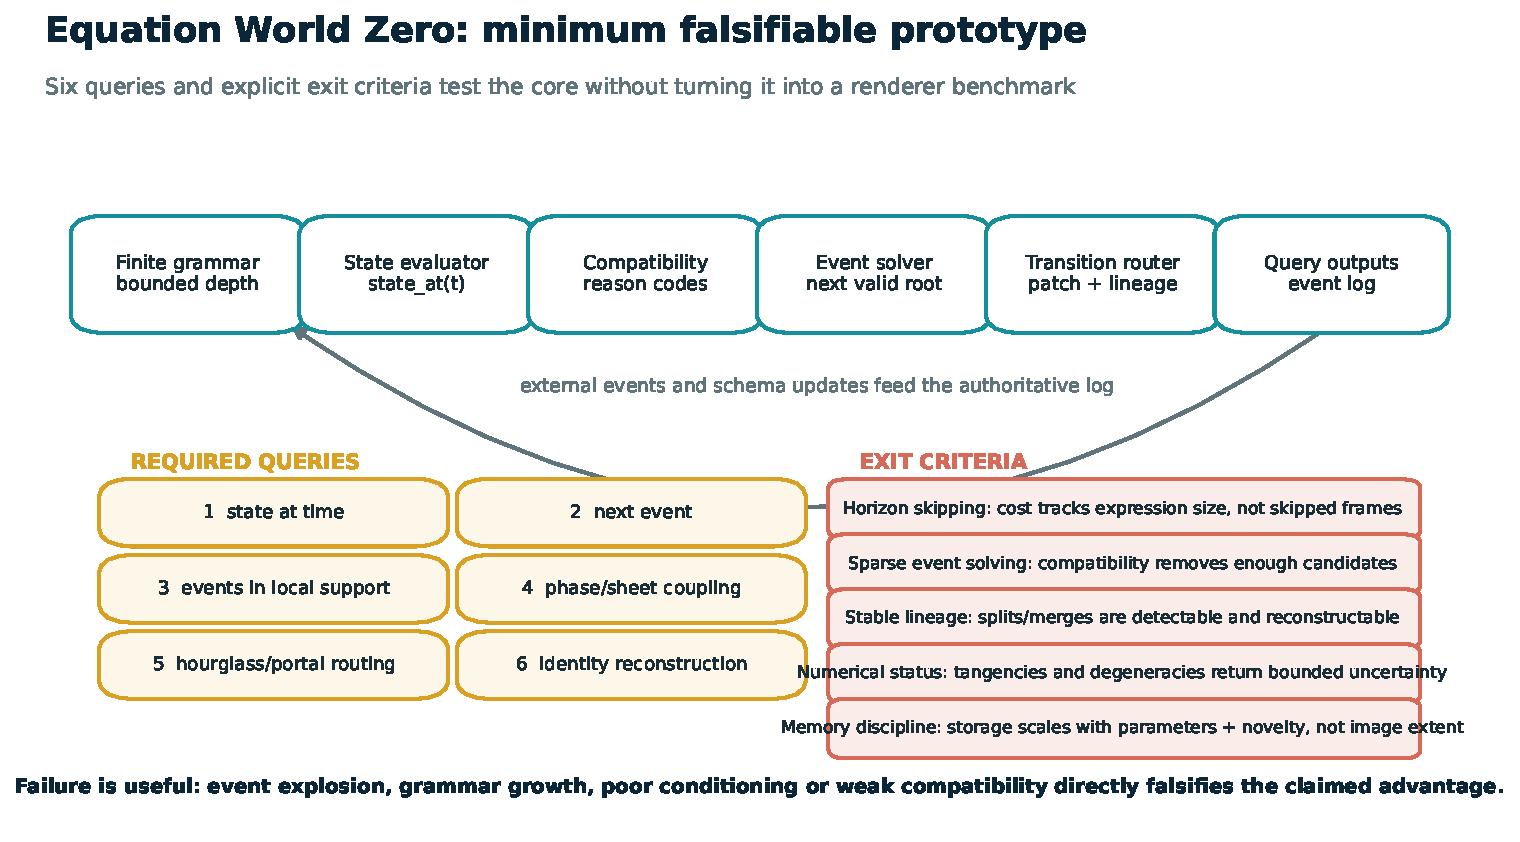
\includegraphics[width=\textwidth]{prototype_flow.pdf}
\caption{Equation World Zero is a bounded falsifiable experiment.}
\end{figure}

\section{Required experiments}
\begin{description}[style=nextline]
\item[Horizon skipping] Measure whether \code{state\_at(t)} depends on expression size rather than the number of skipped frames.
\item[Co-located phase sheets] Verify that same-position states remain uncoupled until explicit compatibility is met.
\item[Event routing] Verify ordering, transition invariants and reason codes at line/circle/hourglass events.
\item[Grammar-depth stress] Measure expression growth and normalization under repeated production.
\item[Identity split/merge] Add explicit parent/merge records and detect lineage collisions.
\item[Minimal agent integration] Let perception and action use the same support/event language without claiming general intelligence.
\end{description}

\section{Failure modes}
The core fails usefully if event density explodes, compatibility filtering is weak, grammar composition escapes the normalized relation family, numerical conditioning is poor, lineage cannot survive split/merge, or exogenous novelty dominates storage.

\section{Implementation roadmap}
\begin{enumerate}
\item Freeze schema version 1.0 and the restricted relation families.
\item Add interval-valued root/status results for tangencies and uncertain coefficients.
\item Add explicit split/merge lineage records and deterministic serialization hashes.
\item Benchmark against fixed-step and conventional CCD baselines at equal error.
\item Integrate one engine adapter with editor visualization but keep authority in the query core.
\item Only after software benchmarks, build Hollowlens-0 with a preregistered electronic baseline.
\end{enumerate}

\chapter{Claims ledger and final decision}
\section{Claims not carried into UGTS-0}
The following are not requirements or conclusions: universal constant-time worlds; zero memory, power, heat or latency; exact non-iterative intersections for arbitrary fields; complete state in one bit; physical Klein-bottle self-assembly; topology that eliminates all broad phase; golden-ratio zero-cost anti-aliasing; replacement of all renderers/PDE solvers; or replacement of general AI.

\begin{longtable}{@{}p{0.07\textwidth}p{0.31\textwidth}p{0.13\textwidth}p{0.43\textwidth}@{}}
\caption{Claims ledger: corrections and rejected totalizing claims.}\label{tab:claims-ledger}\\
\toprule ID & Source claim & Disposition & Technical reason \\ \midrule
\endfirsthead
\multicolumn{4}{l}{\small\itshape Table \ref{tab:claims-ledger} continued}\\
\toprule ID & Source claim & Disposition & Technical reason \\ \midrule
\endhead
\midrule\multicolumn{4}{r}{\small continued on next page}\\\endfoot
\bottomrule\endlastfoot
CL01 & Universal O(1) world/event solving & \statusreject & Only fixed closed expressions and restricted fixed-degree root problems may be horizon-independent; candidate count and solver cost remain. \\
\addlinespace[3pt]
CL02 & Zero memory / under-32MB universal worlds & \statusreject & Parameters can compress some closed dynamics, but entities, branches, exogenous events, calibration and uncertainty consume memory. \\
\addlinespace[3pt]
CL03 & No latency, heat or power & \statusreject & All computation, actuation, detection and display/hardware paths have latency and energy costs. \\
\addlinespace[3pt]
CL04 & One bit contains the complete state & \statusreject & One bit is only a schema-bound flag; numeric state, uncertainty, lineage and parameters remain separate. \\
\addlinespace[3pt]
CL05 & Golden ratio eliminates aliasing at zero cost & \statusdemote & Golden-angle schedules can reduce regularity but require sampling, reconstruction and error analysis. \\
\addlinespace[3pt]
CL06 & Feynman vectors are a standard quantum rasterizer & \statustranslate & Use the phrase only as inspiration; the implementation is complex phasor/oriented supersampling. \\
\addlinespace[3pt]
CL07 & Klein bottle physically self-assembles matter & \statusreject & Use quotient/gluing maps in software; no physical self-assembly claim is supported. \\
\addlinespace[3pt]
CL08 & Möbius strip is simply half a Klein bottle & \statuscorrect & Certain cuts/decompositions relate them, but the statement is not a general unique identity. \\
\addlinespace[3pt]
CL09 & Rows at powers of two in Pascal are all ones/odd & \statuscorrect & With zero-based row indexing, rows 2\textasciicircum{}k-1 are all odd; Pascal parity still yields the Sierpinski pattern. \\
\addlinespace[3pt]
CL10 & C(5,3)=10 proves the decimal threshold relation & \statusdemote & It is a valid combination count and an interesting coincidence, not a causal structural proof. \\
\addlinespace[3pt]
CL11 & Log mapping removes the origin singularity & \statuscorrect & Log mapping relocates/rescales the singular behavior; an epsilon/core chart is still required. \\
\addlinespace[3pt]
CL12 & Analytic SDF intersections are always exact and non-iterative & \statusreject & Only selected field/trajectory pairs have closed-form roots; generic cases need numerical/certified methods. \\
\addlinespace[3pt]
CL13 & All BVH/broad-phase structures become unnecessary & \statusreject & Strong support/compatibility filters may replace or complement broad phase in restricted domains; generic scenes still need indexing. \\
\addlinespace[3pt]
CL14 & The topology solves the Von Neumann bottleneck & \statusreject & Data locality may improve, but instruction/data movement and memory hierarchy remain physical constraints. \\
\addlinespace[3pt]
CL15 & World geometry directly replaces general AI/LLMs & \statusreject & A shared query substrate can host agents, but it does not replace model weights, learning, semantics or inference complexity. \\
\addlinespace[3pt]
CL16 & Biology, dreams, economies and wireless auras instantiate the same exact mechanism & \statusreject & These are narrative analogies in the source bundle, not part of the technical unification. \\
\addlinespace[3pt]
CL17 & Chromatic correction is zero-cost & \statuscorrect & Log-space offsets are cheap, but channel evaluation, filtering, resampling and calibration still cost resources. \\
\addlinespace[3pt]
CL18 & Rasterization and raymarching are forbidden & \statuscorrect & They are optional downstream projection tools; they do not define the authoritative substrate. \\
\addlinespace[3pt]
\end{longtable}


\begin{decisionbox}
\textbf{GO} for formalization and restricted Equation World Zero. Start with algebra of state, support, compatibility, event, transition, identity and memory. Use rasterization, raymarching, game engines and waveguides as downstream adapters or benchmarks. Do not begin by recreating a conventional scene and then mistake the projection for the substrate.
\end{decisionbox}

\appendix
\chapter{Complete extracted concept inventory}
The following table is the comprehensive extraction delivered with the package. The machine-readable version is \path{specs/concept_inventory.csv}.
\begin{landscape}
\begingroup
\scriptsize
\setlength{\tabcolsep}{2pt}
\setlength{\LTleft}{0pt}
\setlength{\LTright}{0pt}
\renewcommand{\arraystretch}{1.10}
\begin{longtable}{@{}L{12mm}L{38mm}L{54mm}L{89mm}L{24mm}L{32mm}@{}}
\caption{Complete extracted concept inventory. ``Source expression'' preserves the corpus framing; ``normalized operator'' is the technical implementation used by UGTS-0.}\label{tab:concept-inventory}\\
\toprule
ID & Category / name & Source expression & Normalized operator and qualification & Status & Source trace \\
\midrule
\endfirsthead
\multicolumn{6}{l}{\small\itshape Table \ref{tab:concept-inventory} continued}\\
\toprule
ID & Category / name & Source expression & Normalized operator and qualification & Status & Source trace \\
\midrule
\endhead
\midrule\multicolumn{6}{r}{\small continued on next page}\\
\endfoot
\bottomrule
\endlastfoot
N01 & \textbf{Radix carry threshold}\par{\tiny\color{UGTSGray} Numeric/fractal} & Digit-count changes at powers of the radix. & Use radix powers as scale/change boundaries and compact level indices.\par{\tiny\color{UGTSGray} Exact for positional number systems.} & \statusretain & {\tiny S1, pp. 1-4} \\
\addlinespace[2pt]
N02 & \textbf{Zero-based offset semantics}\par{\tiny\color{UGTSGray} Numeric/fractal} & An index of 35 denotes the 36th stored position. & Keep value, offset and ordinal position as distinct typed quantities.\par{\tiny\color{UGTSGray} Prevents off-by-one errors; not altered arithmetic.} & \statusretain & {\tiny S4, pp. 1-3} \\
\addlinespace[2pt]
N03 & \textbf{Active-bit/Hamming-weight filter}\par{\tiny\color{UGTSGray} Numeric/fractal} & 19 = 10011 has three active bits; zeros are treated as inactive. & Use popcount as a sparse feature count or seed descriptor.\par{\tiny\color{UGTSGray} The phonetic syllable link is a mnemonic, not a general encoding law.} & \statustranslate & {\tiny S1, pp. 3-5} \\
\addlinespace[2pt]
N04 & \textbf{Three-point triangle seed}\par{\tiny\color{UGTSGray} Numeric/fractal} & Three active positions are treated as triangle anchors. & Map three non-collinear active samples to a simplex/triangle primitive.\par{\tiny\color{UGTSGray} Any three non-collinear points form a triangle; the mapping is chosen.} & \statustranslate & {\tiny S1, pp. 6-7} \\
\addlinespace[2pt]
N05 & \textbf{Pascal parity to Sierpinski}\par{\tiny\color{UGTSGray} Numeric/fractal} & Odd/even entries in Pascal triangle form a Sierpinski pattern. & Use binomial parity as a deterministic fractal/test-pattern generator.\par{\tiny\color{UGTSGray} Technical correction: rows 2\textasciicircum{}k-1, not generally 2\textasciicircum{}k, are all odd when indexed from zero.} & \statusretain & {\tiny S1, pp. 6-9} \\
\addlinespace[2pt]
N06 & \textbf{Golden-angle/Fibonacci sampling}\par{\tiny\color{UGTSGray} Numeric/fractal} & Phi/Vogel spacing is proposed to avoid visible repetition. & Optional quasi-uniform angular sample schedule or dither seed.\par{\tiny\color{UGTSGray} Useful heuristic; it does not guarantee zero aliasing or zero cost.} & \statustranslate & {\tiny S1, pp. 13-15} \\
\addlinespace[2pt]
N07 & \textbf{Lemniscate/strange-loop recursion}\par{\tiny\color{UGTSGray} Numeric/fractal} & Infinity and Escher loops symbolize self-generation. & Represent recursion with explicit finite grammar depth and cycle detection.\par{\tiny\color{UGTSGray} Keep as a recursion motif, not a proof of self-creating physics.} & \statusdemote & {\tiny S1, pp. 18-23} \\
\addlinespace[2pt]
G01 & \textbf{Loop-plus-stem decomposition}\par{\tiny\color{UGTSGray} Glyph/kinematic} & Chosen phi/D/B glyphs are decomposed into loop(s) plus a stem. & Represent glyph geometry as a graph of curve segments and junctions.\par{\tiny\color{UGTSGray} Glyph form varies by font; the decomposition is a design convention.} & \statustranslate & {\tiny S9,S2,S8, pp. 1-2} \\
\addlinespace[2pt]
G02 & \textbf{Cut-unroll D/B to R}\par{\tiny\color{UGTSGray} Glyph/kinematic} & Break the lower loop and straighten the released arc into a diagonal leg. & Boundary-graph edit plus continuous curve morph from closed arc to open segment.\par{\tiny\color{UGTSGray} Implementable as path topology and control-point interpolation.} & \statusretain & {\tiny S9,S2,S8, pp. 1-4} \\
\addlinespace[2pt]
G03 & \textbf{Torque axis T}\par{\tiny\color{UGTSGray} Glyph/kinematic} & The stem is an axis; rotation shears/unreels the lower loop. & Use a rotation/warp parameter around a declared pivot axis.\par{\tiny\color{UGTSGray} Torque language is a kinematic metaphor unless a physical model is supplied.} & \statustranslate & {\tiny S9,S2,S8, pp. 1-4} \\
\addlinespace[2pt]
G04 & \textbf{Delta-time and phase modulation}\par{\tiny\color{UGTSGray} Glyph/kinematic} & Delta T and delta phi drive movement and phase change. & Store continuous time and phase as separate state coordinates and derivatives.\par{\tiny\color{UGTSGray} Do not overload time, torque and triangle into one untyped symbol.} & \statusretain & {\tiny S1,S7,S9, pp. 10-15;14-18;2-5} \\
\addlinespace[2pt]
G05 & \textbf{One-bit parity hinge}\par{\tiny\color{UGTSGray} Glyph/kinematic} & A bit toggles closed/open or route A/B. & Use a schema-bound route/parity flag that selects transition behavior.\par{\tiny\color{UGTSGray} The bit is not the complete state.} & \statusretain & {\tiny S5,S6,S7,S9, pp. 2-8;5-7;14-25;3-8} \\
\addlinespace[2pt]
G06 & \textbf{Global hinge field}\par{\tiny\color{UGTSGray} Glyph/kinematic} & The hinge is applied everywhere through an SDF sign/state change. & Model a global morph or transition field evaluated at every query point.\par{\tiny\color{UGTSGray} A morph parameter changes the implicit field; topology changes require explicit handling.} & \statustranslate & {\tiny S9,S2,S8, pp. 7-8} \\
\addlinespace[2pt]
G07 & \textbf{Chirality/orientation flip}\par{\tiny\color{UGTSGray} Glyph/kinematic} & R/S or mirrored states are associated with sign/orientation reversal. & Track an orientation bit and apply a gluing/transition map that may flip it.\par{\tiny\color{UGTSGray} Orientation is distinct from sheet and phase.} & \statusretain & {\tiny S1,S7,S9, pp. 21-29;18-25;4-8} \\
\addlinespace[2pt]
G08 & \textbf{Split oval to opposing arches}\par{\tiny\color{UGTSGray} Glyph/kinematic} & A zero-centered oval is split and torque opens it into positive/negative wave arches. & Use symmetric curve branches around a fixed node for waveform or deformation profiles.\par{\tiny\color{UGTSGray} The exact 1:1 amplitude condition is a chosen symmetric case, not universal warped-disk physics.} & \statustranslate & {\tiny S4, pp. 10-16} \\
\addlinespace[2pt]
G09 & \textbf{Overlap lens/shared domain}\par{\tiny\color{UGTSGray} Glyph/kinematic} & Slightly overlapping semicircles form an interference/tolerance/shared-information zone. & Use intersection A$\cap$B, lens area, or blend region as explicit shared domain.\par{\tiny\color{UGTSGray} Interpretation depends on geometry, mechanics or information semantics.} & \statusretain & {\tiny S4, pp. 16-19} \\
\addlinespace[2pt]
I01 & \textbf{Signed distance/implicit field}\par{\tiny\color{UGTSGray} Implicit geometry} & Geometry is represented by f(p), with f=0 as the boundary. & Use implicit scalar fields; reserve exact-distance claims for valid primitives/transforms.\par{\tiny\color{UGTSGray} A generic implicit field need not be an exact SDF.} & \statusretain & {\tiny S1,S3,S6,S7,S9, pp. 10-30;1-10;5-10;14-31;7-8} \\
\addlinespace[2pt]
I02 & \textbf{SDF CSG operators}\par{\tiny\color{UGTSGray} Implicit geometry} & Union=min, intersection=max, subtraction=max(a,-b). & Provide composable implicit-field operators with documented sign convention.\par{\tiny\color{UGTSGray} Smooth variants may be added as optional adapters.} & \statusretain & {\tiny S3, pp. 1-3} \\
\addlinespace[2pt]
I03 & \textbf{Zero surface as event relation}\par{\tiny\color{UGTSGray} Implicit geometry} & The SDF-zero locus becomes a transition surface, not a place to march through. & Treat R\_j(q)=0 as an event guard and solve crossing time.\par{\tiny\color{UGTSGray} This is the central correction from rendering to event semantics.} & \statusretain & {\tiny S6,S5,S7, pp. 5-7;3-7;14-31} \\
\addlinespace[2pt]
I04 & \textbf{Analytic kinematic sweep}\par{\tiny\color{UGTSGray} Implicit geometry} & A cone/trajectory is solved against an implicit boundary for exact event time. & Use closed-form roots for restricted trajectory/surface pairs; certified numerical roots otherwise.\par{\tiny\color{UGTSGray} No universal non-iterative solver exists.} & \statusretain & {\tiny S6,S7, pp. 7-12;14-31} \\
\addlinespace[2pt]
I05 & \textbf{Cone as support/domain}\par{\tiny\color{UGTSGray} Implicit geometry} & Cones are directional influence, field-of-view or admissibility domains. & Use analytic radial-angular support predicates for pruning/query scope.\par{\tiny\color{UGTSGray} Not necessarily a rendered cone.} & \statusretain & {\tiny S5,S6,S7, pp. 3-6;5-10;12-25} \\
\addlinespace[2pt]
I06 & \textbf{Spherical/local radial-angular support}\par{\tiny\color{UGTSGray} Implicit geometry} & Spherical means a local chart around a sensor/coupler, not a global world remesh. & Represent local support by radius, angle, orientation, uncertainty and time window.\par{\tiny\color{UGTSGray} Core type-safety rule.} & \statusretain & {\tiny S5,S6, pp. 3-6;1-10} \\
\addlinespace[2pt]
I07 & \textbf{Nested shells}\par{\tiny\color{UGTSGray} Implicit geometry} & Shells organize radial reach, scale and relevance. & Use concentric support bands or multiresolution radial intervals.\par{\tiny\color{UGTSGray} Useful local indexing structure, not required globally.} & \statustranslate & {\tiny S6,S7, pp. 1-7;12-25} \\
\addlinespace[2pt]
I08 & \textbf{Hourglass/quad routing}\par{\tiny\color{UGTSGray} Implicit geometry} & Four conical chambers meet at a pinch/event locus. & Implement a finite routing partition keyed by sign/sheet/orientation at a transition surface.\par{\tiny\color{UGTSGray} The pinch is an event/router, not a literal singularity that destroys data.} & \statustranslate & {\tiny S6,S7, pp. 5-7;23-25} \\
\addlinespace[2pt]
I09 & \textbf{Invariant/eigen-axis}\par{\tiny\color{UGTSGray} Implicit geometry} & A central axis or mode persists through transformations. & Declare invariants and preserved quantities for transitions.\par{\tiny\color{UGTSGray} Eigenlanguage is only literal when a linear operator is actually defined.} & \statusretain & {\tiny S1,S6,S7, pp. 15-20;5-12;18-25} \\
\addlinespace[2pt]
I10 & \textbf{Projective/homogeneous chart}\par{\tiny\color{UGTSGray} Implicit geometry} & Null-cone and projective language compactifies direction/scale. & Optional homogeneous coordinates for intersections and points at infinity.\par{\tiny\color{UGTSGray} Use only where it improves equations and conditioning.} & \statustranslate & {\tiny S6,S7, pp. 5-7;18-25} \\
\addlinespace[2pt]
C01 & \textbf{Log-polar transform}\par{\tiny\color{UGTSGray} Coordinates/sampling} & rho=ln(r), theta=atan2(y,x). & Use a local coordinate chart that turns radial scaling into translation in rho.\par{\tiny\color{UGTSGray} Handle r=0 with an epsilon/core cell.} & \statusretain & {\tiny S1,S3,S7,S9, pp. 10-15;1-10;12-31;5-8} \\
\addlinespace[2pt]
C02 & \textbf{One-bit log-polar LUT}\par{\tiny\color{UGTSGray} Coordinates/sampling} & A bitmask activates radial-angular sectors. & Use as a coarse admission/cache mask, never as the whole world state.\par{\tiny\color{UGTSGray} Schema and quantization parameters are mandatory.} & \statusretain & {\tiny S1,S3,S7,S9, pp. 10-15;1-10;12-31;5-8} \\
\addlinespace[2pt]
C03 & \textbf{Phasor/Feynman-style edge accumulation}\par{\tiny\color{UGTSGray} Coordinates/sampling} & Subpixel samples carry magnitude/phase and are accumulated. & Normalize to complex phasor or oriented coverage accumulation for antialiasing.\par{\tiny\color{UGTSGray} Not a literal Feynman path integral unless a physical path-integral model is defined.} & \statustranslate & {\tiny S3, pp. 1-8} \\
\addlinespace[2pt]
C04 & \textbf{One-bit stochastic jitter}\par{\tiny\color{UGTSGray} Coordinates/sampling} & Binary noise shifts samples/thresholds around an edge. & Use deterministic blue-noise/hash dithering with reproducible seeds.\par{\tiny\color{UGTSGray} Jitter trades structured error for noise; it does not remove error.} & \statusretain & {\tiny S1,S3, pp. 10-15;7-10} \\
\addlinespace[2pt]
C05 & \textbf{Temporal pulse-density modulation}\par{\tiny\color{UGTSGray} Coordinates/sampling} & Brightness/coverage is encoded as density of one-bit pulses. & Optional display-output adapter using PDM or delta-sigma modulation.\par{\tiny\color{UGTSGray} Panel hardware and refresh limits remain.} & \statustranslate & {\tiny S3, pp. 4-6} \\
\addlinespace[2pt]
C06 & \textbf{Chromatic log-radius offset}\par{\tiny\color{UGTSGray} Coordinates/sampling} & Channel scaling becomes additive rho offsets. & Apply channel-specific log-radius shifts before field evaluation, then resample correctly.\par{\tiny\color{UGTSGray} Cheap coordinate arithmetic is not zero-cost end-to-end correction.} & \statusretain & {\tiny S3, pp. 7-8} \\
\addlinespace[2pt]
C07 & \textbf{Log-polar prepress screening}\par{\tiny\color{UGTSGray} Coordinates/sampling} & Spatial one-bit dots scale with rho and orient with theta. & Optional print adapter with calibrated halftone, screen angles and dot-gain compensation.\par{\tiny\color{UGTSGray} Requires press/paper calibration.} & \statustranslate & {\tiny S3, pp. 8-10} \\
\addlinespace[2pt]
T01 & \textbf{Phase sheets}\par{\tiny\color{UGTSGray} Topology} & Multiple states occupy layered sheets over the same base coordinate. & Represent state as base position plus sheet, phase, orientation and address.\par{\tiny\color{UGTSGray} Layer identity must be explicit.} & \statusretain & {\tiny S6,S7,S9, pp. 5-10;14-25;5-8} \\
\addlinespace[2pt]
T02 & \textbf{Double vacuum}\par{\tiny\color{UGTSGray} Topology} & Co-located states do not interact when phase/sheet/address are incompatible. & Compatibility-gated coupling: same x does not imply same sector.\par{\tiny\color{UGTSGray} One of the strongest corpus concepts.} & \statusretain & {\tiny S5,S6,S7, pp. 2-7;5-10;14-25} \\
\addlinespace[2pt]
T03 & \textbf{Mobius gluing}\par{\tiny\color{UGTSGray} Topology} & A boundary identification reverses orientation after one loop. & Implement quotient-map boundary wrapping with orientation flip.\par{\tiny\color{UGTSGray} Use a chart/gluing abstraction rather than literal 4D geometry.} & \statusretain & {\tiny S7,S9, pp. 7-12;5-8} \\
\addlinespace[2pt]
T04 & \textbf{Klein-bottle gluing}\par{\tiny\color{UGTSGray} Topology} & A closed non-orientable quotient is used for looping routes. & Implement two rectangle-edge identifications, one orientation reversing.\par{\tiny\color{UGTSGray} Hardware realization remains frontier; 3D pictures self-intersect.} & \statustranslate & {\tiny S5,S7,S9, pp. 2,5;7-25;5-10} \\
\addlinespace[2pt]
T05 & \textbf{Topological portal/gluing map}\par{\tiny\color{UGTSGray} Topology} & Crossing a boundary re-enters another chart/sheet, possibly transformed. & Use explicit port, orientation map, coordinate transform and transfer metadata.\par{\tiny\color{UGTSGray} This makes topology technically testable.} & \statusretain & {\tiny S5,S6,S7, pp. 2-5;5-12;14-25} \\
\addlinespace[2pt]
T06 & \textbf{Inside/outside sign with schema}\par{\tiny\color{UGTSGray} Topology} & Binary sign denotes interior/exterior or route state. & Bind every bit to a declared schema/version and keep uncertainty separate.\par{\tiny\color{UGTSGray} Raw bits without layout/schema are ambiguous.} & \statusretain & {\tiny S3,S5,S7,S9, pp. 1-10;2-7;14-31;3-8} \\
\addlinespace[2pt]
T07 & \textbf{Strange loop/self-reference}\par{\tiny\color{UGTSGray} Topology} & Escher/Klein motifs suggest systems feeding back into themselves. & Use explicit cycles, fixed points and termination/cycle policies in the grammar/event graph.\par{\tiny\color{UGTSGray} Narrative inspiration only unless formally specified.} & \statusdemote & {\tiny S1,S7,S9, pp. 18-30;7-25;5-10} \\
\addlinespace[2pt]
A01 & \textbf{Finite grammar G}\par{\tiny\color{UGTSGray} Information architecture} & A finite rule set generates relations/structures. & Use bounded-depth typed productions that compile to supported relation primitives.\par{\tiny\color{UGTSGray} Enforce symbol and expression caps.} & \statusretain & {\tiny S6,S7,S9, pp. 1-12;26-31;5-8} \\
\addlinespace[2pt]
A02 & \textbf{State manifold Q}\par{\tiny\color{UGTSGray} Information architecture} & State includes position, time, phase, sheet, address and branch. & Use a typed immutable state record; optional orientation and uncertainty extensions.\par{\tiny\color{UGTSGray} Core data model.} & \statusretain & {\tiny S6, pp. 5-7} \\
\addlinespace[2pt]
A03 & \textbf{Relation family R\_j(q)=0}\par{\tiny\color{UGTSGray} Information architecture} & World geometry/constraints are equations rather than frame snapshots. & Store typed relations with parameters, domains and solver capability metadata.\par{\tiny\color{UGTSGray} Restrict to relation families with known solvers for the prototype.} & \statusretain & {\tiny S6, pp. 5-12} \\
\addlinespace[2pt]
A04 & \textbf{Support predicate C<=0}\par{\tiny\color{UGTSGray} Information architecture} & Only relations inside a declared local support are candidates. & Separate admission/support from geometry and from compatibility.\par{\tiny\color{UGTSGray} Supports analytic pruning.} & \statusretain & {\tiny S5,S6, pp. 3-7;5-12} \\
\addlinespace[2pt]
A05 & \textbf{Compatibility predicate chi}\par{\tiny\color{UGTSGray} Information architecture} & Co-location is insufficient; phase/sheet/mode/time/policy must match. & Compose physical and digital compatibility predicates.\par{\tiny\color{UGTSGray} Return reason codes, not only a bit.} & \statusretain & {\tiny S5,S6, pp. 3-7;5-12} \\
\addlinespace[2pt]
A06 & \textbf{Event time t*}\par{\tiny\color{UGTSGray} Information architecture} & The next event is the earliest supported compatible relation root. & Compute min valid root after t0 with tolerance and confidence.\par{\tiny\color{UGTSGray} Multiple roots and tangencies need policy.} & \statusretain & {\tiny S5,S6, pp. 3-7;5-12} \\
\addlinespace[2pt]
A07 & \textbf{Transition rule T\_j}\par{\tiny\color{UGTSGray} Information architecture} & Crossing an event surface updates sheet/phase/branch/invariants. & Use pure transition functions producing state patches and event records.\par{\tiny\color{UGTSGray} Preserve pre/post states and provenance.} & \statusretain & {\tiny S5,S6, pp. 5-7;5-12} \\
\addlinespace[2pt]
A08 & \textbf{Lineage address}\par{\tiny\color{UGTSGray} Information architecture} & Identity persists by generative address and invariant history. & Use stable entity IDs plus parent/merge ancestry and transition lineage.\par{\tiny\color{UGTSGray} Coordinates are not identity.} & \statusretain & {\tiny S5,S6,S7, pp. 3-12;1-12;26-35} \\
\addlinespace[2pt]
A09 & \textbf{Irreducible external event log}\par{\tiny\color{UGTSGray} Information architecture} & Novel exogenous events must be recorded even when closed dynamics are recomputable. & Event-source only novelty, transitions, confidence and calibration changes.\par{\tiny\color{UGTSGray} No zero-memory claim.} & \statusretain & {\tiny S5,S6, pp. 7-11;1-12} \\
\addlinespace[2pt]
A10 & \textbf{Query-first API}\par{\tiny\color{UGTSGray} Information architecture} & Ask state\_at(t), next\_event, events\_in\_support, coupling and identity. & Expose direct query methods independent of a frame loop.\par{\tiny\color{UGTSGray} Projection is downstream.} & \statusretain & {\tiny S5,S6, pp. 3-12;1-12} \\
\addlinespace[2pt]
A11 & \textbf{Projection adapter}\par{\tiny\color{UGTSGray} Information architecture} & Images are optional outputs, not the authoritative state. & Place raster/raymarch/SDF preview in a replaceable adapter layer.\par{\tiny\color{UGTSGray} Do not mistake the projector for the state space.} & \statusretain & {\tiny S3,S6, pp. 1-10;1-12} \\
\addlinespace[2pt]
A12 & \textbf{Hybrid layer separation}\par{\tiny\color{UGTSGray} Information architecture} & Persistent world state, local sensing and display remain distinct. & Use core/query/projection/hardware modules with explicit interfaces.\par{\tiny\color{UGTSGray} Avoid polar-everything and raster-everything.} & \statusretain & {\tiny S5,S6, pp. 2-12;1-12} \\
\addlinespace[2pt]
A13 & \textbf{Branch and chamber routing}\par{\tiny\color{UGTSGray} Information architecture} & Events route state through branches/sheets/chambers. & Use finite enums and explicit routing tables.\par{\tiny\color{UGTSGray} Avoid implicit magic routing.} & \statusretain & {\tiny S6,S7, pp. 5-12;23-31} \\
\addlinespace[2pt]
A14 & \textbf{Uncertainty/confidence}\par{\tiny\color{UGTSGray} Information architecture} & Verified outputs include error, confidence and calibration. & Attach numeric intervals/confidence and solver status to every event.\par{\tiny\color{UGTSGray} Essential for real systems.} & \statusretain & {\tiny S5,S6, pp. 1-12;8-12} \\
\addlinespace[2pt]
A15 & \textbf{Schema-bound packed data caution}\par{\tiny\color{UGTSGray} Information architecture} & Raw packed bits are meaningless without layout metadata. & Version all bitfields/LUTs and ship schema with data.\par{\tiny\color{UGTSGray} Useful contrast from the COBOL sections.} & \statusretain & {\tiny S2,S8,S9,S5, pp. 27-29;26-28;26-28;7} \\
\addlinespace[2pt]
A16 & \textbf{Agent on shared relation substrate}\par{\tiny\color{UGTSGray} Information architecture} & Perception/action can issue the same support/event queries. & Keep agent integration minimal: queries and transition choices, not universal AI compression.\par{\tiny\color{UGTSGray} Do not claim an LLM is replaced by the geometry.} & \statustranslate & {\tiny S6,S7, pp. 11-12;34-36} \\
\addlinespace[2pt]
K01 & \textbf{Analytic motion component}\par{\tiny\color{UGTSGray} Game technology} & Position/velocity/acceleration are closed-form trajectories. & Entity component stores trajectory coefficients and state patches.\par{\tiny\color{UGTSGray} Supports horizon skipping for fixed formulas.} & \statusretain & {\tiny S6,S7,S4, pp. 7-12;26-31;10-16} \\
\addlinespace[2pt]
K02 & \textbf{Continuous collision/event component}\par{\tiny\color{UGTSGray} Game technology} & Collisions are relation roots under support/compatibility. & Event solver returns ordered crossings with guard semantics.\par{\tiny\color{UGTSGray} Fallback numerical solver is allowed.} & \statusretain & {\tiny S6,S7, pp. 7-12;26-31} \\
\addlinespace[2pt]
K03 & \textbf{Sensor cone component}\par{\tiny\color{UGTSGray} Game technology} & Agent/sensor relevance uses local radial-angular supports. & FOV/range query before relation solving.\par{\tiny\color{UGTSGray} Useful in Unity/Godot/ECS adapters.} & \statusretain & {\tiny S5,S6,S7, pp. 3-9;5-12;12-25} \\
\addlinespace[2pt]
K04 & \textbf{Procedural grammar component}\par{\tiny\color{UGTSGray} Game technology} & L-system/shape grammar generates bounded relation sets. & Compile grammar tokens to primitives, supports and transitions.\par{\tiny\color{UGTSGray} Finite depth and normalization required.} & \statusretain & {\tiny S6,S7,S9, pp. 11-12;26-31;5-8} \\
\addlinespace[2pt]
K05 & \textbf{Topological portal component}\par{\tiny\color{UGTSGray} Game technology} & Mobius/Klein/hourglass routes connect spaces with orientation/sheet changes. & Portal has entry surface, exit transform, sheet map and lineage event.\par{\tiny\color{UGTSGray} Can be rendered conventionally while simulated symbolically.} & \statusretain & {\tiny S5,S6,S7,S9, pp. 2-7;5-12;18-25;5-8} \\
\addlinespace[2pt]
K06 & \textbf{Deterministic network/event replication}\par{\tiny\color{UGTSGray} Game technology} & Seed plus event log reconstructs closed dynamics. & Replicate authoritative events and schema versions, not every visual frame.\par{\tiny\color{UGTSGray} Only works where deterministic formulas are stable across platforms.} & \statustranslate & {\tiny S6, pp. 8-12} \\
\addlinespace[2pt]
K07 & \textbf{Graphics preview component}\par{\tiny\color{UGTSGray} Game technology} & SDF/log-polar/jitter projects core state to pixels. & Optional GPU or CPU preview; no authority over simulation.\par{\tiny\color{UGTSGray} Provides practical game-engine visualization.} & \statusretain & {\tiny S1,S3,S6, pp. 10-15;1-10;9-10} \\
\addlinespace[2pt]
H01 & \textbf{Bounded Compatibility Event (B.C.E.)}\par{\tiny\color{UGTSGray} Hardware endpoint} & A verified event is declared only after support, compatibility and a measured guard crossing. & Reuse the core event schema for a measured optofluidic front end.\par{\tiny\color{UGTSGray} The best-defined physical endpoint in the corpus.} & \statusretain & {\tiny S5, pp. 1-12} \\
\addlinespace[2pt]
H02 & \textbf{Local support -> liquid lens -> mode -> guard}\par{\tiny\color{UGTSGray} Hardware endpoint} & Radial-angular input is tuned, coupled, interfered and thresholded. & Separate optical, fluid, mode and digital-control models.\par{\tiny\color{UGTSGray} Maxwell, Young-Laplace/coupled-mode theory and control logic stay type-separated.} & \statusretain & {\tiny S5, pp. 3-9} \\
\addlinespace[2pt]
H03 & \textbf{Matrix-in-glass}\par{\tiny\color{UGTSGray} Hardware endpoint} & A waveguide mesh implements a calibrated transfer function. & Treat as a measured passive/tunable transfer matrix, not stored imagery.\par{\tiny\color{UGTSGray} Requires calibration and drift tracking.} & \statusretain & {\tiny S5, pp. 2-5} \\
\addlinespace[2pt]
H04 & \textbf{One-bit hardware route flag}\par{\tiny\color{UGTSGray} Hardware endpoint} & Parity denotes admission/route/freshness, not amplitude. & Store amplitudes, thresholds, uncertainty and lineage separately.\par{\tiny\color{UGTSGray} Same type-safety rule as software.} & \statusretain & {\tiny S5, pp. 2-7} \\
\addlinespace[2pt]
H05 & \textbf{Spherical throughput metric}\par{\tiny\color{UGTSGray} Hardware endpoint} & Count verified events/queries per second at a declared error budget. & Report support, compatibility, miss/false rates, energy, latency and drift.\par{\tiny\color{UGTSGray} Not photon flux alone.} & \statusretain & {\tiny S5, pp. 3,6,9-12} \\
\addlinespace[2pt]
H06 & \textbf{Hollowlens-0 demonstrator}\par{\tiny\color{UGTSGray} Hardware endpoint} & Scanned input, tunable liquid coupler, 2x2 interferometer, balanced detectors, digital sidecar. & Prototype only after guard, compatibility, calibration and baseline are preregistered.\par{\tiny\color{UGTSGray} Can fail usefully.} & \statusretain & {\tiny S5, pp. 4,8-10} \\
\addlinespace[2pt]
\end{longtable}
\endgroup
\end{landscape}


\chapter{Reference world schema}
\section{Example world}
The included JSON defines two entities, one line event surface, a local radial-angular support, sheet/phase/tag compatibility, and a transition that toggles sheet, flips orientation, changes branch and adds phase.
\lstinputlisting[language={},caption={UGTS-0 example world}]{../specs/example_world.json}

\section{Schema design rules}
\begin{enumerate}
\item Every bitfield has a declared meaning and schema version.
\item Position, time, phase, sheet, orientation, branch, lineage and uncertainty are distinct.
\item Surface solver family is declared and logged.
\item Projection settings are not authoritative simulation state.
\item External novelty and calibration changes enter the event log.
\end{enumerate}

\chapter{Source notes index}
Per-document notes are shipped under \path{source_notes/}. They identify page-level mechanisms, retained operators and excluded extrapolations. The source PDFs themselves are not copied into the ZIP.

\begin{longtable}{@{}p{0.12\textwidth}p{0.36\textwidth}p{0.44\textwidth}@{}}
\toprule Ref & Note file & Primary contribution \\ \midrule\endhead
S1 & \path{S1_NUM19.md} & Radix thresholds, Hamming weight, triangle seed, Pascal parity, fractal and graphics/topology motif chain.\\
S2 & \path{S2_AUTHOR_DIALOGUE.md} & Duplicate glyph/topology thread plus schema, AR and speculative extensions.\\
S3 & \path{S3_KC_GRAPHICS.md} & Log-polar/SDF/one-bit graphics and prepress adapter.\\
S4 & \path{S4_BEN_BURGER.md} & Zero indexing, split oval and shared overlap lens.\\
S5 & \path{S5_WAVEGUIDE.md} & B.C.E., optofluidic signal path, metrics and kill criteria.\\
S6 & \path{S6_CHRONO_SYNTHESIS.md} & Mature query-first event calculus and feasibility discipline.\\
S7 & \path{S7_HOLLOWLAND.md} & Double vacuum, phase sheets, hourglass, grammar and grand claims.\\
S8 & \path{S8_GEORGE_BUNDLE.md} & Overlapping dialogue bundle; deduplicated.\\
S9 & \path{S9_D_TO_PH.md} & Glyph morph, parity hinge, log-polar/L-system and SDF-global morph.\\
\bottomrule
\end{longtable}

\backmatter
\chapter*{Closing statement}
\addcontentsline{toc}{chapter}{Closing statement}
The corpus's most valuable idea survives only after discipline: geometry defines relations and local supports; topology defines explicit gluing and compatibility sectors; information architecture defines typed state, lineage and event semantics; game technology supplies components and adapters; hardware supplies measurable guards and error budgets. With those boundaries, the material becomes a coherent substrate that can be implemented, tested and falsified.

\end{document}
